% Working notes: damping of breathing vortices (Kennedy & Plunk). Preamble and macros follow
% ep_turbulence_paper/main.tex (lines 1-160 and 190-196) so that the notation matches the long paper.
\documentclass{jpp}

\usepackage{graphicx}
\usepackage{amsmath}
\usepackage{array}
\usepackage{tabularx}
\usepackage{amssymb}
\usepackage{xcolor}
\usepackage{tikz}
\usetikzlibrary{patterns,patterns.meta,decorations.pathreplacing,decorations.pathmorphing}
\usepackage[normalem]{ulem}
\usepackage{placeins}

\setcounter{topnumber}{3}
\setcounter{totalnumber}{4}
\renewcommand{\topfraction}{0.9}
\renewcommand{\textfraction}{0.07}
\renewcommand{\floatpagefraction}{0.8}

\interfootnotelinepenalty=10000

\setlength{\paperwidth}{174mm}
\setlength{\paperheight}{247mm}
\usepackage[colorlinks=true,
            linkcolor=blue!60!black,
            citecolor=blue!60!black,
            urlcolor=blue!60!black,
            setpagesize=false,
            hypertexnames=false]{hyperref}

\usepackage{cleveref}
\crefformat{section}{\S#2#1#3}
\crefformat{subsection}{\S#2#1#3}
\crefformat{subsubsection}{\S#2#1#3}
\crefformat{figure}{figure~#2#1#3}
\crefformat{equation}{(#2#1#3)}
\crefrangeformat{equation}{(#3#1#4)--(#5#2#6)}
\crefrangeformat{figure}{figures #3#1#4--#5#2#6}
\def\closesymbol{\!}
\newcommand{\order}[1]{O\left(#1\right)}
\newcommand{\orderinline}[1]{O(#1)}
\newcommand{\rmd}{\text{d}}

\newcommand{\bv}{\mathbf{v}}
\newcommand{\br}{\mathbf{r}}
\newcommand{\bB}{\mathbf{B}}

\ifdefined\closesymbol
	\relax
\else
	\def\closesymbol{\relax}
\fi

\newcommand{\pt}{\partial_t}
\newcommand{\px}{\partial_x}
\newcommand{\py}{\partial_y}
\newcommand{\pz}{\partial_z}

\ifdefined\partd
	\renewcommand{\partd}[3][]{\frac{{\partial^{#1} #2}}{{\partial #3}^{#1}}}
\else
	\newcommand{\partd}[3][]{\frac{{\partial^{#1} #2}}{{\partial #3}^{#1}}}
\fi

\ifdefined\vec
	\renewcommand{\vec}[1]{\boldsymbol{#1}}
\else
	\newcommand{\vec}[1]{\boldsymbol{#1}}
\fi

\newcommand{\uvec}[1]{\hat{\boldsymbol{#1}}}
\providecommand{\bcdot}{\vec{\cdot}}

\newcommand{\grad}{{\vec{\nabla}}}
\ifdefined\div
	\renewcommand{\div}{{\grad\bcdot}}
\else
	\newcommand{\div}{{\grad\bcdot}}
\fi

\ifdefined\vr
	\renewcommand{\vr}{{\vec{r}}}
\else
	\newcommand{\vr}{{\vec{r}}}
\fi
\newcommand{\vp}{{\vec{p}}}
\newcommand{\vq}{{\vec{q}}}
\newcommand{\vk}{{\vec{k}}}

\ifdefined\vv
	\renewcommand{\vv}{{\vec{v}}}
\else
	\newcommand{\vv}{{\vec{v}}}
\fi

\newcommand{\vkperp}{{\vk_\perp}}
\newcommand{\kperp}{k_\perp}
\newcommand{\kpar}{k_\parallel}
\newcommand{\vperp}{v_\perp}
\newcommand{\vvperp}{\vv_\perp}
\newcommand{\vpar}{v_\parallel}
\newcommand{\hvpar}{\hat v_\parallel}

\newcommand{\intr}[1][3]{{\int \rmd^{#1} \vec{r} \ }}
\newcommand{\intR}[1][3]{{\int \rmd^{#1} \vec{R} \ }}
\newcommand{\intv}[1][3]{{\int \rmd^{#1} \vec{v} \ }}
\newcommand{\intw}[1][3]{{\int \rmd^{#1} \vec{w} \ }}


\newcommand{\s}{s}
\newcommand{\vth}{v_\text{th}}
\newcommand{\vths}{v_{\text{th}\s}}
\newcommand{\vthi}{v_{\text{th}i}}
\newcommand{\vthe}{v_{\text{th}e}}
\newcommand{\mfp}{\lambda_\text{mfp}}
\newcommand{\ope}{\omega_{\text{p}e}}
\newcommand{\lDe}{\lambda_{\text{D}e}}
\newcommand{\rhoi}{\rho_i}
\newcommand{\rhoe}{\rho_e}
\newcommand{\rhos}{\rho_s}

\newcommand{\fs}{f_{\s}}
\newcommand{\fos}{f_{0\s}}
\newcommand{\Fs}{F_{\s}}
\newcommand{\Fos}{F_{0\s}}
\newcommand{\dfs}{\delta \closesymbol f_{\s}}

\newcommand{\fe}{f_{e}}
\newcommand{\foe}{f_{0e}}
\newcommand{\Fe}{F_{e}}
\newcommand{\Foe}{F_{0e}}
\newcommand{\dfe}{\delta \closesymbol f_{e}}

\newcommand{\fion}{f_{i}}
\newcommand{\foi}{f_{0i}}
\newcommand{\Fi}{F_{i}}
\newcommand{\Foi}{F_{0i}}
\newcommand{\dfi}{\delta \closesymbol f_{i}}

\newcommand{\kperprhoisq}{\kperp^2\rhoi^2}
\newcommand{\kperprhoisqq}{\kperp^4\rhoi^4}
\newcommand{\kperprhoesq}{\kperp^2\rhoe^2}
\newcommand{\kperprhoesqq}{\kperp^4\rhoe^4}
\newcommand{\pbra}[2]{\left\lbrace #1, #2 \right\rbrace}
\newcommand{\pbrainline}[2]{\lbrace #1, #2 \rbrace}

\newcommand{\vR}{{\vec{R}}}
\newcommand{\vE}{\vec{E}}
\newcommand{\vB}{\vec{B}}
\newcommand{\exb}{\(\vE\times\vB\)}

\newcommand{\avgR}[1]{\left\langle #1 \right\rangle_\vec{R}}
\newcommand{\avgRs}[1]{\left\langle #1 \right\rangle_{\vec{R}_\s}}
\newcommand{\avgRinline}[1]{\langle #1 \rangle_\vec{R}}
\newcommand{\avgr}[1]{\left\langle #1 \right\rangle_{\vec{r}}}
\newcommand{\avgrinline}[1]{\langle #1 \rangle_\vec{r}}

	
\emergencystretch=3em
\raggedbottom
\newcommand{\lambdaD}{\lambda_D}
\newcommand{\debye}{\lambda_D^2}
\newcommand{\omstar}{\omega_*}
\newcommand{\omd}{\omega_d}
\newcommand{\Zhat}{\hat{Z}}
\newcommand{\lavg}[1]{\langle #1 \rangle_\lambda}
\newcommand{\gene}{\texttt{GENE}}

% ---------------------------------------------------------------------------
% Additional cleveref formats and notes-specific macros
% ---------------------------------------------------------------------------
\Crefformat{equation}{Equation~(#2#1#3)}
\Crefformat{figure}{Figure~#2#1#3}
\crefformat{table}{table~#2#1#3}
\Crefformat{table}{Table~#2#1#3}
\crefformat{appendix}{Appendix~#2#1#3}
\Crefformat{appendix}{Appendix~#2#1#3}
\crefformat{footnote}{footnote~#2#1#3}
\crefmultiformat{equation}{(#2#1#3)}{ and~(#2#1#3)}{, (#2#1#3)}{ and~(#2#1#3)}
\crefmultiformat{section}{\S#2#1#3}{ and~\S#2#1#3}{, \S#2#1#3}{ and~\S#2#1#3}
\crefmultiformat{subsection}{\S#2#1#3}{ and~\S#2#1#3}{, \S#2#1#3}{ and~\S#2#1#3}
\crefmultiformat{figure}{figures~#2#1#3}{ and~#2#1#3}{, #2#1#3}{ and~#2#1#3}
\crefrangeformat{section}{\S\S#3#1#4--#5#2#6}
\usepackage{booktabs}

\newcommand{\phibar}{\bar\phi}
\newcommand{\varphibar}{\bar\varphi}
\newcommand{\rme}{\text{e}}
\newcommand{\rmi}{\text{i}}
\newcommand{\vda}{\bar v_{da}}
\newcommand{\nz}{\text{nz}}
\newcommand{\zon}{\text{zon}}
\newcommand{\Enz}{E_\text{nz}}
\newcommand{\Ezon}{E_\text{zon}}
\newcommand{\Znz}{Z_\text{nz}}
\newcommand{\Wnz}{W_\text{nz}}
\newcommand{\GammaE}{\Gamma_{\!E}}
\newcommand{\gammaamp}{\gamma_\text{amp}}
\newcommand{\omtr}{\omega_\text{tr}}
\newcommand{\omb}{\omega_\text{b}}
\newcommand{\wt}{\tilde\omega}
\newcommand{\Lop}{\mathcal{L}}
\newcommand{\Nop}{\mathcal{N}}
\newcommand{\Ham}{\mathcal{H}}
\newcommand{\Kfn}{\mathcal{K}}
\newcommand{\Zfn}{\mathcal{Z}}
\newcommand{\Dfn}{\mathcal{D}}
\newcommand{\Pk}{\mathcal{P}}
\newcommand{\PV}{\operatorname{PV}}
\newcommand{\Cxy}{C_{xy}}
\newcommand{\dx}{\Delta x}
\newcommand{\Omstar}{\Omega_*}
\newcommand{\what}{\hat\omega_d}

\shorttitle{Damping of breathing vortices: working notes}
\shortauthor{D. Kennedy and G.G. Plunk}

\title{Damping of breathing vortices in a dipole pair-plasma condensate: working notes}

\author{D.~Kennedy$^{1}$\thanks{Email address for correspondence: daniel.kennedy@ukaea.uk}
  \and G.G.~Plunk$^{2}$}

\affiliation{$^{1}$UKAEA (United Kingdom Atomic Energy Authority), Culham Campus, Abingdon, Oxfordshire, OX14 3DB, UK\\
$^{2}$Max-Planck-Institut f\"ur Plasmaphysik, Greifswald, Germany}

\begin{document}

\maketitle

\begin{abstract}
The two box-scale vortices which breathe on the zonal condensate of a strongly driven, temperature-gradient-dominated dipole pair plasma do not persist: in a reduced-box simulation, they decay, ever faster, until they collapse. In these working notes, we give the theory of their existence and of their decay, and test it against the simulation. The vortices are the shear-flow instability of their own jets. In the fluid limit of the kinetic equations, the jets and the vortices obey the two-dimensional Euler equation; jets whose shear layers are corrugated at the Debye scale are unstable, in the sense of Rayleigh, to perturbations of the scale of the box; and the instability saturates when the fluid at its critical layers is trapped. Rayleigh's equation on the measured jets predicts the frequency and the radial structure of the vortices, and their amplitude obeys the trapping law, viz., the trapping frequency is a constant multiple of the Rayleigh growth rate, while their energy falls by orders of magnitude. The vortices are damped kinetically: the part of their potential that is not flute-like does work on particles streaming along the field line, and this Landau damping converts their electrostatic energy into entropy at a rate that does not depend on their amplitude. The jets make up for the loss as long as they are unstable. The vortices therefore decay at the rate at which their jets lose their instability, and collapse when the jets become stable. We close by listing what remains open, in particular the rate at which the corrugation of the jets is eroded, and the simulations, now running, that bear on it.
\end{abstract}

% ===========================================================================
\section{Introduction}\label{sec:intro}
% ===========================================================================

Strongly driven electron--positron plasmas in a dipole collapse, after a single explosive burst of interchange activity, into a box-scale zonal condensate on which two coherent vortices ride, one on each jet, carried in opposite directions and exchanging electrostatic energy with the zonal flow at twice their advection frequency --- the `breathing' of \citet{KennedyPlunkLetter}. Nothing in the collisionless transit-averaged model damps the flute-like zonal part of this state \citep{KennedyPlunkManuscript, KennedyPlunkLetter}, and the net injection of free energy by the gradients is negligible; the condensate is therefore long-lived, and the transport it carries is close to zero. The vortices, however, are not protected in the same way: in a reduced-box simulation of the same state, their energy falls slowly for several thousand time units, then ever faster, until they collapse into a weak, partly incoherent remnant. Coherent structures riding on sheared flows are common in zonally dominated plasma turbulence \citep{Ivanov2020, Ivanov2025}, and their lifetime can be as important as their existence. Since the vortices carry the large oscillating fluxes of the condensate, what removes them --- and whether it would also remove them in a less idealised plasma --- determines the long-time state of the system.

The vortices are the shear-flow instability of their own jets. The zonal flow of the condensate is not a single harmonic: its shear layers are corrugated at the scale of the Debye length, and such jets are unstable, in the sense of \citet{Rayleigh1880}, to perturbations of the scale of the box. The instability saturates when the fluid at its critical layers is trapped in cat's eyes \citep{ONeil1965, Stewartson1978, WarnWarn1978}, and the saturated state is the pair of breathing vortices. This state is not lossless, however. A vortex is flute-like only at scales larger than the Debye length; the small part of its potential that varies along the field line does work on the particles that stream along it, and this Landau damping \citep{Landau1946} converts the electrostatic energy of the vortex into fine structure in velocity space, at a rate that does not depend on its amplitude. The jets make up for the loss, since the vortices draw on them, but only as long as the jets remain unstable, and the corrugation that makes them so is itself slowly eroded. The vortices therefore decay at the rate at which their jets lose their instability, and collapse when the jets become stable. This picture is sketched in \cref{fig:cartoon}.

\begin{figure}
\centering
% Cartoon of how the vortices lose energy (TikZ; \input from notes.tex inside a figure environment).
% Colours as in the data figures: grey = zonal flow, orange = exchange with the jets, green = conversion to entropy,
% red = the velocity-space sink.
\definecolor{cjet}{gray}{0.45}
\definecolor{csup}{HTML}{FF7F0E}
\definecolor{cent}{HTML}{2CA02C}
\definecolor{crem}{HTML}{D62728}
\begin{tikzpicture}[x=1cm, y=1cm, >=stealth, line cap=round, line join=round]
% ---------------------------------------------------------------- (a) geometry
\begin{scope}[xscale=0.88]
  \node[anchor=north west] at (-0.62, 6.55) {(a)};
  % zonal flow profile and phase speed
  \draw[cjet, line width=1.4pt] plot[domain=0:5.6, samples=60] (\x, {5.35 + 0.62*cos(deg(2*pi*(\x-2.8)/5.6))});
  \draw[densely dashed] (0, 5.598) -- (5.6, 5.598);
  \node[anchor=west, cjet] at (3.25, 6.12) {$U(x)$};
  \node[anchor=west] at (4.75, 5.83) {$c$};
  \fill (1.767, 5.598) circle (1.4pt); \fill (3.833, 5.598) circle (1.4pt);
  % the (x, y) plane
  \draw[black!35] (0, 0) rectangle (5.6, 4.2);
  \begin{scope}
    \clip (0, 0) rectangle (5.6, 4.2);
    % critical layers
    \draw[densely dotted] (1.767, 0) -- (1.767, 4.2); \draw[densely dotted] (3.833, 0) -- (3.833, 4.2);
    % cat's eyes: one per wavelength on each flank, staggered by half a wavelength (the shear changes sign)
    \foreach \yc in {2.1}
      \filldraw[fill=csup!14, draw=black, line width=0.8pt] (1.767, \yc-1.75) .. controls (2.30, \yc-0.75) and (2.30, \yc+0.75) .. (1.767, \yc+1.75)
        .. controls (1.234, \yc+0.75) and (1.234, \yc-0.75) .. cycle;
    \foreach \yc in {0, 4.2}
      \filldraw[fill=csup!14, draw=black, line width=0.8pt] (3.833, \yc-1.75) .. controls (4.366, \yc-0.75) and (4.366, \yc+0.75) .. (3.833, \yc+1.75)
        .. controls (3.300, \yc+0.75) and (3.300, \yc-0.75) .. cycle;
    % trapped orbits
    \draw[black!55, line width=0.4pt] (1.767, 2.1) ellipse (0.20 and 0.95);
    \draw[black!55, line width=0.4pt] (3.833, 0) ellipse (0.20 and 0.95); \draw[black!55, line width=0.4pt] (3.833, 4.2) ellipse (0.20 and 0.95);
    % open streamlines: the jet core and the two outer regions
    \foreach \xo/\am in {2.52/-0.13, 2.80/-0.13, 3.08/-0.13}
      \draw[cjet, line width=0.5pt] plot[domain=0:4.2, samples=40] ({\xo + \am*cos(deg(2*pi*\x/4.2))}, \x);
    \foreach \xo/\am in {0.38/0.05, 0.86/0.14}
      \draw[cjet, line width=0.5pt] plot[domain=0:4.2, samples=40] ({\xo + \am*cos(deg(2*pi*\x/4.2))}, \x);
    \foreach \xo/\am in {4.74/0.14, 5.22/0.05}
      \draw[cjet, line width=0.5pt] plot[domain=0:4.2, samples=40] ({\xo + \am*cos(deg(2*pi*\x/4.2))}, \x);
  \end{scope}
  % links between the profile and the plane
  \draw[densely dotted] (1.767, 4.2) -- (1.767, 5.598); \draw[densely dotted] (3.833, 4.2) -- (3.833, 5.598);
  % labels
  \draw[->, cjet, line width=1.3pt] (2.93, 1.50) -- (2.93, 2.70);
  \draw[<->, line width=0.5pt] (1.367, 2.1) -- (2.167, 2.1);
  \node[fill=csup!14, inner sep=1pt] at (1.767, 2.42) {$2w$};
  \draw[->] (0, -0.3) -- (1.0, -0.3) node[anchor=west] {$x$};
  \draw[->] (-0.3, 0) -- (-0.3, 1.0) node[anchor=south] {$y$};
  \node[anchor=north] at (3.6, -0.08) {critical layers, $U = c$};
\end{scope}
% ---------------------------------------------------------------- (b) energy flow
\begin{scope}[xshift=5.95cm,
    box/.style={draw, rounded corners=2pt, line width=0.7pt, align=center, inner sep=4pt, minimum height=1.05cm}]
  \node[anchor=north west] at (-0.15, 6.55) {(b)};
  \node[box, draw=cjet, line width=1.2pt, minimum width=1.7cm] (J) at (0.95, 5.05) {jets\\$E_\mathrm{zon}$};
  \node[box, minimum width=1.7cm] (V) at (5.55, 5.05) {vortices\\$E_\mathrm{nz}$};
  \node[box, draw=cent, minimum width=3.2cm] (F) at (4.80, 2.05) {fine structure in\\velocity space, $Z_\mathrm{nz}$};
  % exchange with the jets
  \draw[->, csup, line width=1.6pt] ([yshift=6pt]J.east) -- node[above, text=black, align=center] {momentum of\\the damping} ([yshift=6pt]V.west);
  \draw[<-, csup!55!black, line width=1.6pt] ([yshift=-6pt]J.east) -- node[below, text=black] {Reynolds stress} ([yshift=-6pt]V.west);
  % kinetic removal
  \draw[->, cent, line width=1.6pt] (V.south) -- (V.south |- F.north);
  \node[anchor=east, align=right] at (5.35, 3.55) {Landau damping of\\the non-flute part, at a\\rate independent of\\amplitude};
  \draw[->, crem, line width=1.6pt, decorate, decoration={snake, amplitude=1.2pt, segment length=6pt, post length=4pt}] (F.south) -- ++(0, -0.9);
  \node[anchor=north] at (4.80, 0.50) {velocity-space sink};
\end{scope}
\end{tikzpicture}

\caption{A cartoon of how the vortices lose their energy. (a) The geometry: the zonal flow \(U(x)\) of one jet (grey, top) and the phase speed \(c\) of its vortex (dashed), which cross at two critical layers on the flanks of the jet (dotted); below, the streamlines in the frame of the vortex, with a cat's eye of trapped fluid, of half-width \(w\), at each critical layer, the two rows of eyes staggered by half a wavelength, and the jet (grey arrow) meandering between them. (b) The flow of energy: while the vortices are large, the jets feed them (solid orange arrow), because the vortices are the shear instability of the jets; the electrostatic energy \(\Enz\) of the vortices is converted into entropy \(\Znz\), i.e., fine structure in velocity space, by phase mixing along the field line (green arrow), at a rate that does not depend on their amplitude, and removed there by the velocity-space sink (red arrow); once the jets have become stable, the exchange reverses (dashed orange arrow) and the vortices collapse.}
\label{fig:cartoon}
\end{figure}

In these notes, we first summarise the setting in \cref{sec:setting}, viz., the transit-averaged equations, the strongly driven condensate and the reduced-box simulation with its restarts. In \cref{sec:theory}, we derive the theory: the fluid limit and the instability of the jets (\cref{sec:euler,sec:rayleigh}), its saturation by trapping (\cref{sec:pendulum}), the kinetic loss (\cref{sec:loss}) and the decay that results from the three together (\cref{sec:decay}). In \cref{sec:data}, we test each of these against the simulation. \Cref{sec:summary} summarises what is established and what is open. The derivations are given step by step in \cref{app:rayleigh,app:trapping,app:landau}.

% ===========================================================================
\section{The setting}\label{sec:setting}
% ===========================================================================

In this section, we recall the equations of \citet{KennedyPlunkLetter} and \citet{KennedyPlunkManuscript} to the extent needed here, describe the strongly driven condensate in which the vortices live, and specify the simulations analysed in \cref{sec:data}.

\subsection{Transit-averaged equations}\label{sec:equations}

We consider a symmetric electron--positron plasma, with charges \(e_p = -e_e = e\), a common Maxwellian \(f_0\) of density \(n_0\) and temperature \(T\), in the ordering \(\rho \ll \lambdaD \ll L\), where \(\rho\) is the Larmor radius, \(\lambdaD = \sqrt{\epsilon_0 T/2n_0e^2}\) the Debye length and \(L\) an equilibrium length. We use flux coordinates \((\psi, \alpha, l)\) with \(\vB = \grad\psi\times\grad\alpha\), and write \(\delta f_a = h_a - e_a\phi f_0/T\). Below the transit and bounce frequencies, \(h_a(\psi,\alpha,\varepsilon,\lambda,t)\) is independent of \(l\) \citep{Helander2014, MPH2018}, where \(\varepsilon = mv^2/2\) is the energy and \(\lambda = v_\perp^2/Bv^2\) the pitch-angle variable, and particles respond to the orbit-averaged potential
\begin{equation}
\phibar(\lambda) = \frac{1}{\hat\tau(\lambda)}\int_{l_1}^{l_2}\frac{\phi(l)\,\rmd l}{\sqrt{1-\lambda B(l)}},
\qquad
\hat\tau(\lambda) = \int_{l_1}^{l_2}\frac{\rmd l}{\sqrt{1-\lambda B(l)}},
\label{eq:orbit}
\end{equation}
where \(l_1\) and \(l_2\) are the bounce points of a trapped particle or the ends of one field-line period for a passing one. To leading order in \(\kperp\rho\), the kinetic and field equations are \citep{Abel2013, MPH2018, KennedyPlunkManuscript}
\begin{align}
\pt h_a + \pbra{\phibar}{h_a} + \vda\,\partial_\alpha h_a
&= \frac{e_af_0}{T}\left(\pt\phibar - v_{*a}^{T}\,\partial_\alpha\phibar\right),\label{eq:kinetic}\\
\left(1-\lambdaD^2\nabla_\perp^2\right)\frac{e\phi}{T}
&= \frac{1}{2n_0}\int\rmd^3\vv\,(h_p-h_e),\label{eq:poisson}
\end{align}
where \(\pbrainline{X}{Y} \equiv \partial_\psi X\,\partial_\alpha Y - \partial_\alpha X\,\partial_\psi Y\) is the \exb{} advection, \(\vda\) is the orbit-averaged binormal magnetic drift, which is energy dependent and of opposite sign for the two species, and \(v_{*a}^{T} = -(T/e_a)\,\partial_\psi\ln f_0\) is the gradient drive at fixed energy. The dipole has no radial magnetic drift, so the zonal flow suffers no collisionless damping.

The nonlinearity of \cref{eq:kinetic} conserves the free energy \(W\) and the electrostatic energy \(E\) separately, and their difference \(Z = W - E \geq 0\) is the entropy of the orbit-averaged perturbation \citep{KennedyPlunkManuscript, KennedyPlunkLetter}; these invariants are the closed-field-line counterparts of those of two-dimensional gyrokinetics \citep{Plunk2010, PlunkTatsuno2011}. Here, we need only two further facts. Firstly, the free energy obeys
\begin{equation}
\frac{\rmd W}{\rmd t} = P - D,
\label{eq:balance}
\end{equation}
where \(P\) is the injection by the gradients and \(D \geq 0\) is the irreversible removal, which, in the simulations, is entirely due to hyperdiffusion \citep{KrommesHu1994, Sugama1996}. Secondly, if we split \(E = \Ezon + \Enz\) into its zonal (\(k_y = 0\)) and non-zonal parts, the nonlinear transfer between the two satisfies
\begin{equation}
\left(\pt\Ezon\right)_\text{NL} = -\left(\pt\Enz\right)_\text{NL},
\label{eq:exchange}
\end{equation}
i.e., the zonal flow and the vortices exchange electrostatic energy without loss; this exchange is the breathing \citep{KennedyPlunkLetter}. We shall write \(\Znz\) and \(\Wnz = \Enz + \Znz\) for the non-zonal parts of \(Z\) and \(W\), and \(\GammaE \equiv -\rmd\ln\Enz/\rmd t\) for the decay rate of the non-zonal electrostatic energy. For a structure of fixed shape, \(\GammaE = 2\gammaamp\), where \(\gammaamp\) is the decay rate of its amplitude.

\subsection{The strongly driven condensate}\label{sec:condensate}

At \(\eta \equiv L_n/L_T = 1\), the drive is above the fluid-interchange threshold \citep{MPH2018}, and the interchange grows at the same rate at every wavelength the box allows. A single \(k_y = 1\) streamer then collapses, in one burst, into \(k_x = 1\) zonal bands, viz., one jet in each direction across the periodic box, modulated by two box-scale vortices, one on each jet \citep{KennedyPlunkLetter}. The two vortices move in opposite directions, related by the symmetry of the pair-plasma equations under exchange of the species together with \(\phi\to-\phi\) and \(y\to-y\), and their relative phase sets the tilt of the flow between them, so the exchange \cref{eq:exchange} runs at \(\omb = 2|\omega_\text{adv}|\), twice the advection frequency of either vortex. Over a breathing cycle, the state changes little; over many cycles, the vortices decay. In what follows, we call \(k_y = 1\) the vortex and \(k_y = 0\) the jet, and the question of these notes is why the former decays while the latter does not.

\subsection{The reduced-box simulation and its restarts}\label{sec:runs}

All the data in these notes comes from one nonlinear simulation with the gyrokinetic code \gene{} \citep{Jenko2000} in the dipole flux tube of \citet{KennedyPlunkLetter}, at \(\eta = 1\), started from noise, in a box a quarter of the production box in each perpendicular direction, together with restarts of it. Its parameters are collected in \cref{tab:runs}. There is no collision operator: all irreversible removal is by fourth-order hyperdiffusion, spectral in \(x\) and \(y\) [rate \(\nu_\perp(\dx\,k_x/2)^4\), where \(\dx\) is the radial grid spacing, and likewise in \(y\)], and by finite-difference hyperdiffusion along the field line and in \(v_\parallel\). One property of the grid will matter in \cref{sec:collapse}: the radial grid spacing is comparable with the Debye length, \(\lambdaD\approx1.2\,\dx\). The run is continued for many thousands of breathing periods after the burst, until long after the vortices have disappeared. Times are in \(L_\text{ref}/c_\text{ref}\), lengths in \(\rho_\text{ref}\), and energies in the units of the \gene{} free-energy diagnostics \citep{BanonNavarro2011, BanonNavarro2016}.

\begin{table}
\centering
\begin{tabular}{lll}
\toprule
Quantity & Symbol & Value \\
\midrule
Gradient drives & \(\omega_n = \omega_T\) & \(2.7816\) (\(\eta = 1\)) \\
Grid & \(n_{x0}\times n_{ky0}\times n_{z0}\) & \(64\times16\times32\) \\
Velocity grid & \(n_v\), \(L_v\) & \(84\), \(4.5\) \\
Box & \(L_x\), \(k_{y,\text{min}}\) & \(3689\,\rho_\text{ref}\), \(2\times10^{-3}\,\rho_\text{ref}^{-1}\) \\
Debye length & \(\lambdaD\) & \(70.7\,\rho_\text{ref} = 1.23\,\dx\) \\
Perpendicular hyperdiffusion & \(\nu_x = \nu_y\) & \(2.4\times10^{-3}\) (spectral, fourth order) \\
Parallel hyperdiffusion & \(\nu_z\) & \(0.05\) (fourth order) \\
Velocity-space hyperdiffusion & \(\nu_v\) & \(0.2\) (fourth order in \(v_\parallel\)) \\
Collisions & --- & none \\
\bottomrule
\end{tabular}
\caption{A summary of the parameters of the reduced-box simulation analysed in these notes. The restarts share them, except where stated otherwise.}
\label{tab:runs}
\end{table}

The first two restarts, which we call the \textit{amplitude tests}, start from a checkpoint of the original run in the slow phase of the decay, with every \(k_y \geq 1\) component of the distribution function multiplied by \(\epsilon = 0.3\) or \(\epsilon = 0.03\) and the zonal component left untouched; the potential follows from \cref{eq:poisson}. Each is run for a few hundred breathing periods. These restarts ask what a vortex does when it is made smaller on unchanged jets.

Five further restarts start from a later checkpoint, in the accelerating phase of the decay, and change one thing each: the velocity-space hyperdiffusion or the perpendicular hyperdiffusion, multiplied or divided by four, or the radial resolution, doubled at fixed box size and fixed hyperdiffusion coefficient. Since the perpendicular hyperdiffusion is normalised to the grid, the last of these also weakens the radial hyperdiffusion at a given physical wavenumber, by a factor of sixteen: it is a test of the grid scale against the Debye scale, not a convergence test. These restarts are running at the time of writing, and only the questions that they are to answer appear in these notes.

% ===========================================================================
\section{Theory of the vortices}\label{sec:theory}
% ===========================================================================

In this section, we derive the three elements of the picture of \cref{fig:cartoon}, viz., the instability of the jets, its saturation and the kinetic loss, and then put them together.

\subsection{The fluid limit}\label{sec:euler}

At the scale of the box, the jets and the vortices are flute-like, and the magnetic drift is slow compared with their motion. In this limit, the kinetic problem collapses to a fluid one, as the following argument shows; the steps are given in \cref{app:rayleigh_moment}.

Let us take the charge moment \(\sum_a e_a\intv\) of \cref{eq:kinetic} with \(\phibar = \phi\). The bracket commutes with the velocity integral, the gradient drive cancels between the species because \(e_a\,(e_af_0/T)\,v_{*a}^T = -e_a\,\partial_\psi f_0\) sums to zero, and the drift term survives only through the even part \(h_p + h_e\), since \(e_a\vda\) is the same for both species. Using \cref{eq:poisson} to write the charge moment as \((2n_0e^2/T)(1-\lambdaD^2\nabla_\perp^2)\phi\), and \(\pbrainline{\phi}{\phi} = 0\), we find\footnote{Strictly speaking, \cref{eq:euler} holds as written in a flux tube whose metric is constant along the field line; in the dipole, \(\nabla_\perp^2\) depends on \(l\), and a flute-like \(\phi\) satisfies it only on average along the line. This is consistent with the approximate flute-like character of the long-wavelength states \citep{KennedyPlunkManuscript}. In the flux tube of the simulations, the average is weighted by the Jacobian, and its effect on \cref{eq:rayleigh} is to replace \(k^2\) in the Laplacian by \(k^2\langle g^{yy}\rangle/\langle g^{xx}\rangle\), where \(g^{xx}\) and \(g^{yy}\) are the metric coefficients; this correction is of order unity, and the stability of the jets depends on it (\cref{sec:unstable}).}
\begin{equation}
\pt\nabla_\perp^2\phi + \pbra{\phi}{\nabla_\perp^2\phi} = \frac{T}{2n_0e\lambdaD^2}\,\partial_\alpha\intv\bar v_{dp}\left(h_p + h_e\right),
\label{eq:euler}
\end{equation}
where \(\bar v_{dp}\) is the positron drift. The right-hand side is smaller than the terms on the left by the ratio of the drift speed to the speed of the vortex relative to the flow, and we neglect it from here on. What remains is the two-dimensional Euler equation for the streamfunction \(\phi\) and the vorticity \(\nabla_\perp^2\phi\): the Debye length drops out, the gradients drop out, as they do for a symmetric pair plasma in a straight field \citep{Helander2014}, and the system of jets and vortices is an incompressible inviscid flow. Two properties of this limit matter in what follows. Firstly, the vortices and the jets can exchange electrostatic energy, by \cref{eq:exchange}, but neither can lose it. Secondly, nothing in it refers to the amplitude of the gradients that drive the turbulence in which the condensate was born: the vortices are a property of the jets.

\subsection{The instability of the jets}\label{sec:rayleigh}

Let \(U \equiv \partial_\psi\Phi\) be the velocity of a zonal flow with potential \(\Phi(\psi)\).\footnote{Not to be confused with the specific flux-tube volume \(U = \oint\rmd l/B\) of \citet{KennedyPlunkLetter}, which does not appear in these notes.} Linearising the Euler equation about it, with \(\phi = \Phi + \varphi(\psi)\,\rme^{\rmi k\alpha - \rmi\omega t}\), where real parts are understood, and writing \(c \equiv \omega/k\) for the phase speed, gives Rayleigh's equation \citep{Rayleigh1880, DrazinReid2004},
\begin{equation}
\left(U - c\right)\left(\partial_\psi^2 - k^2\right)\varphi - U''\varphi = 0,
\label{eq:rayleigh}
\end{equation}
in which \(U''\) is the gradient of the zonal vorticity.\footnote{In the flux tube of the simulations, \(k^2\) in the Laplacian of \cref{eq:rayleigh} is replaced by \(k^2\langle g^{yy}\rangle/\langle g^{xx}\rangle\), where the angle brackets denote the average along the field line of the metric coefficients (\cref{app:rayleigh_metric}).} The surfaces on which \(U = c\) are the critical layers of the perturbation: there, the perturbation is at rest in the frame of the fluid, \cref{eq:rayleigh} is singular, and the perturbation exchanges energy with the mean flow. For a perturbation whose growth rate \(\gamma_\text{R}\) is small compared with its frequency, the exchange at the critical layers determines the growth rate \citep{Briggs1970},
\begin{equation}
\gamma_\text{R} = \pi\,\frac{\sum_c U''_c\,|\varphi_c|^2/|U'_c|}{\partial_{\omega_r}\PV\!\int\rmd\psi\,k\,U''|\varphi|^2/(\omega_r - kU)},
\label{eq:gamma_rayleigh}
\end{equation}
where \(k > 0\), the sum runs over the critical layers, the subscript \(c\) denotes evaluation there, \(\omega_r\) is the real part of the frequency, and \(\PV\) denotes the principal value. Whether the perturbation grows or decays thus depends on the gradient of the zonal vorticity at its critical layers. This is the content of Rayleigh's theorem: a flow can be unstable only if \(U''\) changes sign. The derivation of \cref{eq:rayleigh,eq:gamma_rayleigh} and the proof of the theorem are given in \cref{app:rayleigh_equation,app:rayleigh_theorem,app:rayleigh_growth}.

Two cases concern us. A jet that consists of a single harmonic of the box, in a box that is shorter in the direction of the flow than across it, is stable. A jet of the same amplitude whose shear layers are corrugated, so that each is split into strips of vorticity and \(U''\) changes sign close to the critical layers, is unstable. The first is the zonal flow of the condensate as it would be without structure at the Debye scale; the second is the zonal flow that the simulations have (\cref{sec:unstable}).

\subsection{Saturation by trapping}\label{sec:pendulum}

A growing vortex changes the trajectories of the fluid at its critical layers, and this is what stops its growth. We use local coordinates \((x, y)\), radial and binormal, and the \exb{} streamfunction \(\Psi\).\footnote{In \gene{} units, \(\Psi = \phi/\Cxy\) with \(\Cxy\) the metric factor of the flux tube, \(x\) is in \(\rho_\text{ref}\) and \(t\) in \(L_\text{ref}/c_\text{ref}\). \gene{} writes the real field as \(\phi = \phi_0 + 2\operatorname{Re}(\phi_{k_y}\rme^{\rmi k_yy})\), so the cosine amplitude of a single \(k_y\) is \(A = 2|\phi_{k_y}|/\Cxy\).} In the frame \(\xi = y - ct\) that moves with the vortex, the flow is steady, and the trajectories are the level lines of the Hamiltonian
\begin{equation}
\dot x = -\partial_\xi\Ham,
\qquad
\dot\xi = \partial_x\Ham,
\qquad
\Ham = \Psi_\zon(x) + \Psi_v(x,\xi) - cx,
\label{eq:hamiltonian}
\end{equation}
where \(\Psi_\zon\) and \(\Psi_v\) are the streamfunctions of the jet and of the vortex. Let \(x_c\) be a critical layer, \(U(x_c) = c\), with shear \(S \equiv U'(x_c)\), and let \(A\) be the amplitude of the vortex there. Expanding \cref{eq:hamiltonian} about \(x_c\) gives the Hamiltonian of a pendulum,
\begin{equation}
\Ham = \text{const} + \frac{S}{2}X^2 - A\cos(k\xi) + \dots,
\qquad
X = x - x_c.
\label{eq:pendulum}
\end{equation}
The fluid within a distance \(w\) of the critical layer is trapped: it circulates on closed streamlines, the `cat's eye' of Kelvin, at the frequency \(\omtr\), where
\begin{equation}
\omtr = |k|\sqrt{|S|A},
\qquad
w = 2\sqrt{\frac{A}{|S|}},
\label{eq:trapping}
\end{equation}
are the frequency of small oscillations about the centre of the eye and the half-width of its separatrix (\cref{app:trapping_pendulum}); both scale as \(A^{1/2}\). On the two flanks of a jet, the shear has opposite signs, and the eyes are staggered by half a wavelength (see \cref{fig:cartoon}).

The growth rate \cref{eq:gamma_rayleigh} assumes that the fluid crosses the critical layer on its unperturbed trajectory. Once the fluid there has been trapped and has turned over, i.e., after a time of order \(1/\omtr\), the vorticity inside the cat's eye has been rearranged and the exchange with the mean flow ceases \citep{ONeil1965, Stewartson1978, WarnWarn1978}. An instability that grows at the rate \(\gamma_\text{R}\) therefore saturates when the trapping frequency has become a fixed multiple of the growth rate,
\begin{equation}
\omtr = \alpha\,\gamma_\text{R},
\qquad\text{i.e.,}\qquad
A = \frac{\alpha^2\gamma_\text{R}^2}{k^2|S|},
\label{eq:saturation}
\end{equation}
where \(\alpha\) is a pure number, which this argument does not determine (\cref{app:trapping_saturation}). If the jets change slowly compared with \(\omtr\), the vortex stays at this level and its amplitude follows the growth rate: a vortex on jets that slowly lose their instability decays, and it disappears when they become stable.

\subsection{The kinetic loss}\label{sec:loss}

In the fluid limit, the vortices lose nothing. What they do lose, they lose through the part of their potential that is not flute-like. A flute-like potential cannot satisfy \cref{eq:poisson} everywhere on a field line along which \(\kperp\) varies: the potential must vary along the line by an amount that is proportional to the potential itself and increases steeply with \(\kperp\lambdaD\), becoming of order unity at the Debye scale \citep{KennedyPlunkLetter}. A potential that varies along the field line has a parallel electric field, and this field does work on the particles that stream along the line in resonance with it, viz., those whose transit or bounce frequency matches the frequency \(\omega - kU\) of the vortex in the frame of the local flow. This is Landau damping \citep{Landau1946}. It converts electrostatic energy into fine structure in \(v_\parallel\), i.e., into entropy, at the rate
\begin{equation}
L = 2\gamma_\parallel f\,\Enz,
\label{eq:loss}
\end{equation}
where \(f\) is the fraction of the energy of the vortices that resides in the non-flute part of their potential and \(\gamma_\parallel\), of the order of the transit frequency, is the rate at which that part is damped (see \cref{app:landau}).

Three properties of \cref{eq:loss} are worth noting. Firstly, the loss is linear in the energy of the vortices, so its rate \(L/\Enz\) does not depend on their amplitude. Secondly, it is not affected by trapping, which concerns the motion across the field, not along it. Thirdly, since \(f\) increases steeply with \(\kperp\lambdaD\), the loss is weaker the larger the vortices are compared with the Debye length. The transit-averaged equations of \cref{sec:equations} do not contain this loss, because they assume that particles sample the whole field line many times in one period of the perturbation, whereas the frequency of a vortex relative to the flow of its jet is not small compared with the transit frequency. The entropy that the loss produces is removed by whatever dissipates fine structure in velocity space: collisions in a real plasma, and velocity-space hyperdiffusion in the simulations.

\subsection{The decay}\label{sec:decay}

Let us now put these elements together. The electrostatic energy of the vortices obeys
\begin{equation}
\frac{\rmd\Enz}{\rmd t} = T - L,
\label{eq:budget}
\end{equation}
where \(T\) is the nonlinear transfer of electrostatic energy from the jets to the vortices, i.e., the average of the exchange \cref{eq:exchange} over the breathing. The loss \(L\) is given by \cref{eq:loss}. The transfer \(T\) is not free: since the amplitude of the vortices is held at the saturated level \cref{eq:saturation}, the vortices draw from their jets what they lose, and no more. They do so at the expense of the corrugation that makes the jets unstable, which is also eroded directly by any dissipation that acts on fine zonal structure. As the corrugation is eroded, \(\gamma_\text{R}\) falls, and, by \cref{eq:saturation}, the energy of the vortices falls with it, as \(\gamma_\text{R}^4\). When the jets become stable, the exchange at the critical layers changes sign, as \cref{eq:gamma_rayleigh} does, the jets absorb what the Landau damping leaves, and the vortices collapse.

The theory thus makes the following predictions, which we test in \cref{sec:data}: (i)~the vortices have the frequency and the radial structure of the unstable mode of Rayleigh's equation on their jets; (ii)~their trapping frequency is a constant multiple of the growth rate of that mode, however much either changes; (iii)~a vortex that is reduced in amplitude on unchanged jets regrows; (iv)~the vortices lose electrostatic energy to entropy at a rate that does not depend on their amplitude, through the streaming of particles along the field line; (v)~the jets supply the vortices with energy while they are unstable, less as they become less unstable, and absorb energy from them once they are stable; and (vi)~a two-dimensional fluid with the same jets has the same vortices, but lacks their kinetic loss.

% ===========================================================================
\section{Comparison with the simulations}\label{sec:data}
% ===========================================================================

We now test the predictions of \cref{sec:decay} against the reduced-box simulation and its restarts (\cref{sec:runs}). All measurements of the potential are made at the outboard mid-plane, and, as in \cref{sec:condensate}, \(k_y = 1\) denotes the vortices and \(k_y = 0\) the jets. The two counter-propagating vortices are separated by a two-frequency least-squares fit, \(a_+\rme^{-\rmi\omega_+t} + a_-\rme^{-\rmi\omega_-t}\), in windows of about sixteen breathing periods.

\subsection{The decay}\label{sec:observations}

The energy \(\Enz\) of the vortices falls by orders of magnitude between the burst and their collapse [see \cref{fig:history}(a)]. The decay is not exponential. After a relaxation that follows the burst, the rate \(\GammaE\) passes through a broad minimum and then increases, ever faster, until the vortices collapse [see \cref{fig:history}(b)]. Throughout, the zonal energy \(\Ezon\) decays at a rate that is smaller than \(\GammaE\) by orders of magnitude, and the net injection \(P\) is negligible.

\begin{figure}
\centering
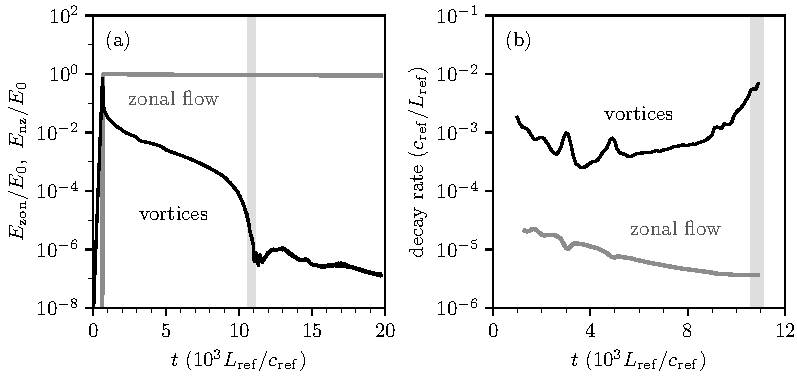
\includegraphics{figures/history.pdf}
\caption{Electrostatic energy of the zonal flow and of the vortices in the reduced-box simulation. (a) The zonal energy \(\Ezon\) (grey) and the non-zonal energy \(\Enz\) (black), as running means over about ten breathing periods, in units of \(E_0\), the largest value of \(\Ezon\). (b) The decay rates \(\GammaE = -\rmd\ln\Enz/\rmd t\) (black) and \(-\rmd\ln\Ezon/\rmd t\) (grey), from least-squares fits of the logarithm of each energy in sliding windows of about a hundred breathing periods, from the end of the relaxation that follows the burst to the end of the collapse. The grey band marks the collapse in this and all subsequent figures. The vortices lose many decades of energy, ever faster and without a plateau, and then collapse, while the zonal flow barely changes.}
\label{fig:history}
\end{figure}

A vortex that is made smaller on unchanged jets does two things (see \cref{fig:amplitude}). It first regrows, relative to its rescaled initial energy, the more so the smaller it was made; it then decays faster than the original, at a rate close to that which the original run reaches when it has itself decayed to the same amplitude. The first is the instability of the jets (\cref{sec:saturated}); the second is the dependence of the exchange with the jets on amplitude (\cref{sec:dissipation}).

\begin{figure}
\centering
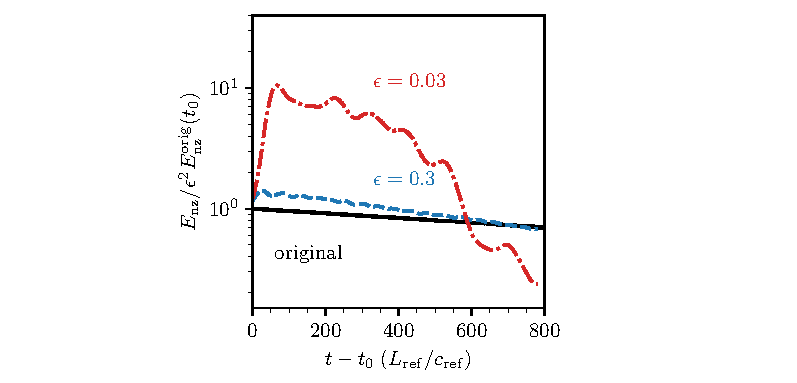
\includegraphics{figures/amplitude.pdf}
\caption{The amplitude tests. (a) The non-zonal electrostatic energy of the original run (black solid) and of the restarts with \(\epsilon = 0.3\) (blue dashed) and \(\epsilon = 0.03\) (red dash-dotted), divided by \(\epsilon^2\) and by the energy of the original run at the restart time \(t_0\), as running means over about ten breathing periods. (b) The decay rate \(\GammaE\) against the amplitude measure \(a = (\Enz/\Ezon)^{1/2}\), which decreases to the right: the original run (black line; fits in windows of about a hundred breathing periods, from the end of the relaxation that follows the burst to the collapse) and the restarts after their regrowth (blue squares and red triangles; windows half as long). A vortex that is made smaller on unchanged jets first regrows and then decays faster than before; the weaker the vortices, the faster they decay.}
\label{fig:amplitude}
\end{figure}

\subsection{The vortices and their critical layers}\label{sec:geometry}

Each vortex propagates in the direction of its own jet, at a fixed fraction of the peak speed of the jet [see \cref{fig:geometry}(a)]. It is radially broad --- a plateau over its own jet, with maxima on both flanks --- and its maxima lie just inside its critical layers, where the shear is near its largest. The streamlines of the moving-frame Hamiltonian \cref{eq:hamiltonian} show the cat's eyes directly, one on each flank of the jet, staggered by half a wavelength [see \cref{fig:geometry}(b)].

\begin{figure}
\centering
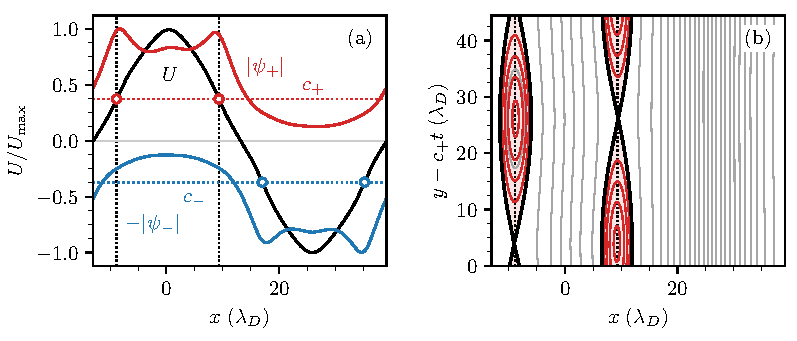
\includegraphics{figures/geometry.pdf}
\caption{Geometry of the vortices on the zonal jets, at one time in the slow phase of the decay. (a) The zonal flow \(U\) (black), normalised to its maximum, and the radial profiles of the two vortices, \(|\psi_+|\) (red) and \(-|\psi_-|\) (blue), each normalised to its own maximum; the horizontal dotted lines are the phase speeds \(c_\pm\) of the two vortices in the same normalisation, the open circles mark the critical layers \(U = c_\pm\), and the vertical dotted lines mark those of the \(+\) vortex. (b) Streamlines of the moving-frame Hamiltonian \cref{eq:hamiltonian} of the \(+\) vortex, with \(\vda = 0\) and the \(-\) vortex left out (grey); the separatrices are drawn in heavy black, and the trapped orbits inside them in red. The radial coordinate is shifted by a quarter of the box so that neither jet is cut by the periodic boundary. Each vortex sits on its own jet, its critical layers lie on the flanks of that jet, not at its maximum, and a cat's eye several Debye lengths wide forms at each of them.}
\label{fig:geometry}
\end{figure}

Two premises of \cref{sec:theory} can be checked at once. Firstly, at the wavenumber of the vortices, the drift frequency of a thermal particle\footnote{Here the magnetic drift is the one that the code applies, viz., the curvature and \(\grad B\) drift of its geometry, averaged along the field line.} is smaller than the frequency of the vortex relative to the flow of its jet by orders of magnitude, and it displaces the resonance of a thermal particle from the critical layer by a small fraction of a grid cell, whereas the cat's eyes are several grid cells wide. The drift is therefore negligible for the motion of the vortices. Secondly, the breathing modulates the jets by a relative amount of the order of \(\Enz/\Ezon\), which is small, so the jets may be treated as steady in \cref{eq:rayleigh}.

\subsection{The vortices are the unstable mode of their jets}\label{sec:unstable}

Rayleigh's equation \cref{eq:rayleigh}, with the field-line-averaged metric of the flux tube, has one unstable mode in each direction on the measured zonal flow. Its frequency follows that of the vortices throughout the run, while both change substantially, and its radial structure is that of the vortices [see \cref{fig:rayleigh}(b,c)]. This is prediction (i). The reason for the instability is visible in the zonal vorticity: each shear layer between the jets is split into two strips, so that \(U''\) changes sign close to each critical layer, and the critical layers sit on the strips [see \cref{fig:rayleigh}(a)]. A single harmonic of the same amplitude is stable; it is the corrugation of the jets at the Debye scale that makes them unstable. The formula \cref{eq:gamma_rayleigh} gives the growth rate of the unstable mode closely. The growth rate falls slowly during the decay and vanishes at the collapse [see \cref{fig:rayleigh}(d)].

\begin{figure}
\centering
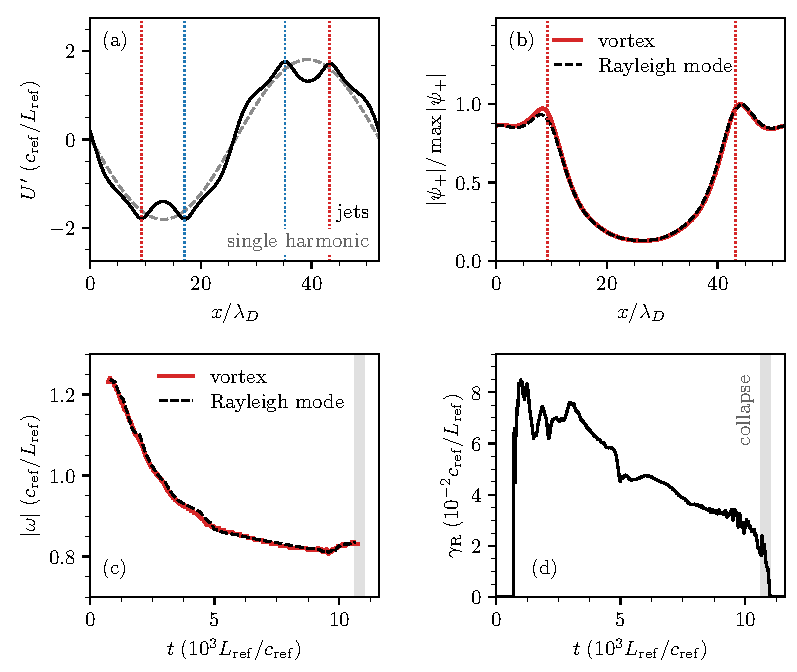
\includegraphics{figures/rayleigh.pdf}
\caption{The vortices as the shear-flow instability of the jets. (a) The zonal vorticity \(U'\) of the measured jets (black) and of a single harmonic of the same amplitude (grey dashed), at one time in the slow phase of the decay; the vertical dotted lines mark the critical layers \(U = \pm c\) of the vortex \(+\) (red) and \(-\) (blue). (b) The radial structure of the vortex \(+\) (red) and of the unstable mode of Rayleigh's equation \cref{eq:rayleigh} on the same jets (black dashed). (c) The frequency of the vortices (red) and of the unstable Rayleigh mode on the measured jets (black dashed) through the run. (d) The growth rate \(\gamma_\text{R}\) of that mode; the grey band marks the collapse. The vortices are the unstable shear mode of jets whose shear layers have split into vorticity strips, and they disappear when that instability does.}
\label{fig:rayleigh}
\end{figure}

\subsection{The vortices are saturated by trapping}\label{sec:saturated}

\Cref{fig:saturation} tests prediction (ii), the saturation law \cref{eq:saturation}, with \(\omtr\) measured from the vortices and \(\gamma_\text{R}\) computed from the jets, two independent inputs. The law holds through the whole decay of the original run, including the collapse, with a single value of \(\alpha\), while the energy of the vortices falls by orders of magnitude. The amplitude tests are a more demanding check, since they change \(\omtr\) on given jets. Both restarts regrow, which is prediction (iii), at a rate comparable with the Rayleigh growth rate [see \cref{fig:euler}(b)]. The \(\epsilon = 0.3\) restart regrows onto the curve of the original run and stays there. The \(\epsilon = 0.03\) restart, whose cat's eyes are no wider than a grid cell, stays below it: its jets lose their instability before it has regrown to the saturated level [see \cref{fig:saturation}(b)]. We conclude that \cref{eq:saturation} describes the vortices as long as their cat's eyes are resolved; the data would also admit a somewhat steeper dependence on \(\gamma_\text{R}\) than the linear one.

\begin{figure}
\centering
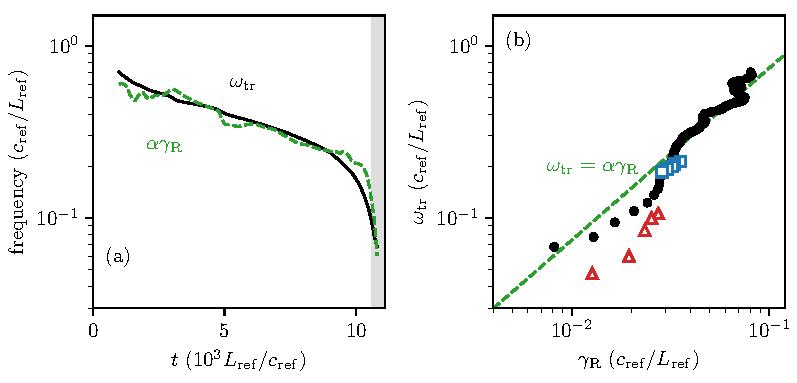
\includegraphics{figures/saturation.pdf}
\caption{The saturation law \cref{eq:saturation}. (a) The trapping frequency \(\omtr\) of the vortices, from \cref{eq:trapping} at their critical layers (black), and the growth rate \(\gamma_\text{R}\) of the unstable Rayleigh mode of the measured jets, multiplied by the constant \(\alpha\) (green dashed), both as means over about eighty breathing periods; \(\alpha\) is the geometric mean of their ratio, and the grey band marks the collapse. (b) The same data, \(\omtr\) against \(\gamma_\text{R}\) (black dots), with the line \(\omtr = \alpha\gamma_\text{R}\), and the \(\epsilon = 0.3\) (blue squares) and \(\epsilon = 0.03\) (red triangles) restarts, with \(\gamma_\text{R}\) computed on their own jets. The growth rate is that of the inviscid problem, converged in radial resolution. The amplitude of the vortices follows the growth rate of the instability of their jets: the vortices decay because the jets become stable.}
\label{fig:saturation}
\end{figure}

\subsection{The energy budget of the vortices}\label{sec:dissipation}

The free-energy diagnostics of \gene{} \citep{BanonNavarro2011} resolve every term of the energy balance in \((k_x, k_y)\) and separate the electrostatic energy from the entropy, so both terms of the budget \cref{eq:budget} can be measured (see \cref{fig:exchange}).\footnote{All rates in this subsection are averages over the breathing, which the output resolves with only about three samples per period; the mean is fitted together with two harmonics of \(\omb\), and the scatter between consecutive windows gives the errors shown in \cref{fig:exchange}. The direct action of the perpendicular sink on \(\Enz\) is negligible until the collapse.}

\begin{figure}
\centering
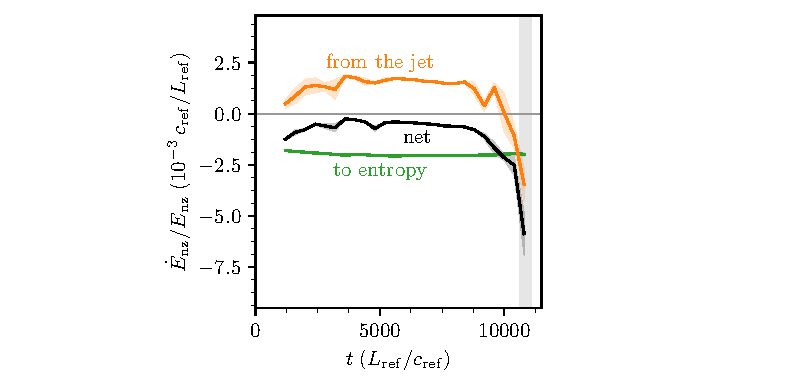
\includegraphics{figures/exchange.pdf}
\caption{The budget \cref{eq:budget} of the electrostatic energy of the vortices, averaged over the breathing. (a) The rates of change of \(\Enz\), per unit \(\Enz\), due to the nonlinear exchange with the zonal flow, \(T/\Enz\) (orange), due to the linear terms, which convert electrostatic energy into entropy, \(-L/\Enz\) (green), and their sum (black); the bands are standard errors over consecutive windows, and the grey band marks the collapse. (b) The exchange \(T/\Enz\) against the amplitude measure \(a = (\Enz/\Ezon)^{1/2}\), which decreases to the right, for the original run (black dots) and for the \(\epsilon = 0.3\) (blue square) and \(\epsilon = 0.03\) (red triangles) restarts; the dotted line is the magnitude of the loss. The vortices lose electrostatic energy to entropy at a steady rate that does not depend on their amplitude; the jets replace most of it while they are unstable, and the decay accelerates because that supply fades and finally reverses.}
\label{fig:exchange}
\end{figure}

The loss rate \(L/\Enz\) is constant while the energy of the vortices falls by orders of magnitude, and it is the same in the amplitude tests as in the original run: the loss is linear in the energy of the vortices. Nearly all of it is carried by the streaming of particles along the field line, and the small remainder by the magnetic drift (see \cref{fig:channels}); and it is smaller in the production run, whose vortices are larger compared with the Debye length. This is prediction (iv).\footnote{The comparison with the production run is only indicative: that run has not yet run far beyond its burst, and its vortices are larger, relative to their jets, than any in the reduced box.}

\begin{figure}
\centering
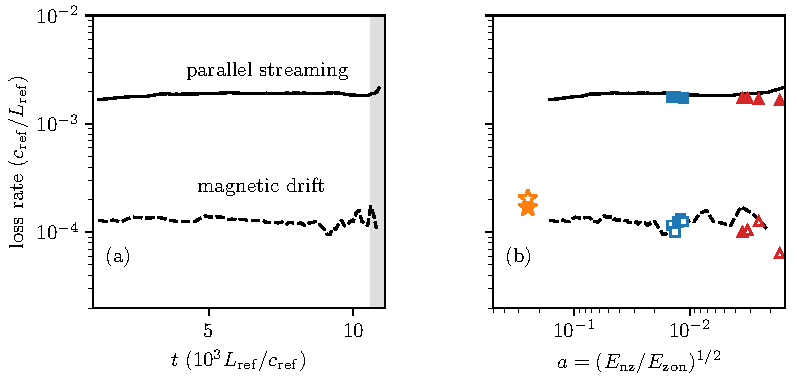
\includegraphics{figures/channels.pdf}
\caption{The channels through which the vortices lose electrostatic energy to entropy. (a) The rate of loss of \(\Enz\), per unit \(\Enz\), through the streaming of particles along the field line (solid) and through the magnetic drift (dashed), in sliding windows of about a hundred breathing periods of the original run; the grey band marks the collapse. (b) The same two rates against the amplitude measure \(a = (\Enz/\Ezon)^{1/2}\), which decreases to the right, for the original run (lines) and the \(\epsilon = 0.3\) (squares) and \(\epsilon = 0.03\) (triangles) restarts, with filled symbols for the streaming and open ones for the drift, and for the production run of \citet{KennedyPlunkLetter}, whose box is four times larger in each perpendicular direction (stars). The loss is carried by the streaming of particles along the field line, at a rate that does not depend on the amplitude of the vortices and is smaller in the larger box.}
\label{fig:channels}
\end{figure}

The part of the potential of the vortices that varies along the field line, which is what does the work, is shown in \cref{fig:flute}. It is a negligible fraction of their power at the scale of the box, grows steeply with the radial wavenumber, and saturates at a value of order unity for \(k_x\lambdaD\gtrsim1\), in the slow phase of the decay and before the collapse alike. With the fraction \(f\) so measured and a damping rate \(\gamma_\parallel\) of the order of the transit frequency, \cref{eq:loss} gives the order of magnitude of the measured loss. The entropy so produced is removed by the velocity-space hyperdiffusion, which accounts for most of the free energy removed from the non-zonal part [see \cref{fig:dissipation}(b)]; the perpendicular sink, by contrast, acts almost entirely on the zonal flow, at a rate that the vortices do not affect [see \cref{fig:dissipation}(a)].

\begin{figure}
\centering
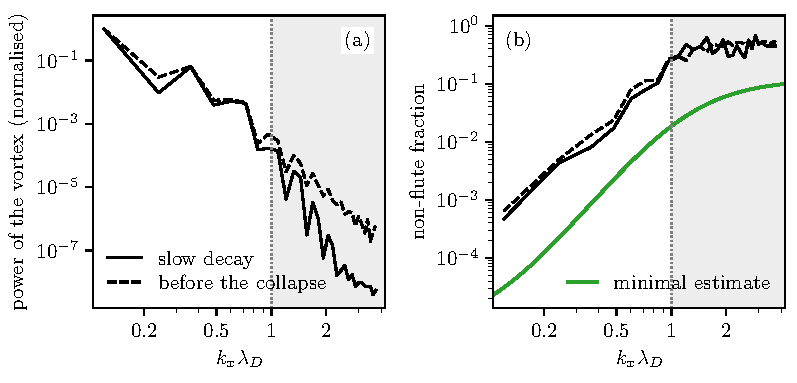
\includegraphics{figures/flute.pdf}
\caption{Flute character of the vortices, scale by scale. (a) The power of the \(k_y = 1\) potential, summed along the field line and averaged over all output times in the slow phase of the decay (solid line) and in the approach to the collapse (dashed line), against the radial wavenumber \(k_x\lambdaD\), each normalised to its maximum. (b) The fraction of that power that is not flute-like, i.e., the power of the departure of the potential from its mean along the field line divided by the total, for the same two intervals. The vertical dotted line marks \(k_x\lambdaD = 1\), and scales smaller than the Debye length are shaded. The vortices are flute-like at the scale of the box and lose their flute character at the Debye scale.}
\label{fig:flute}
\end{figure}

\begin{figure}
\centering
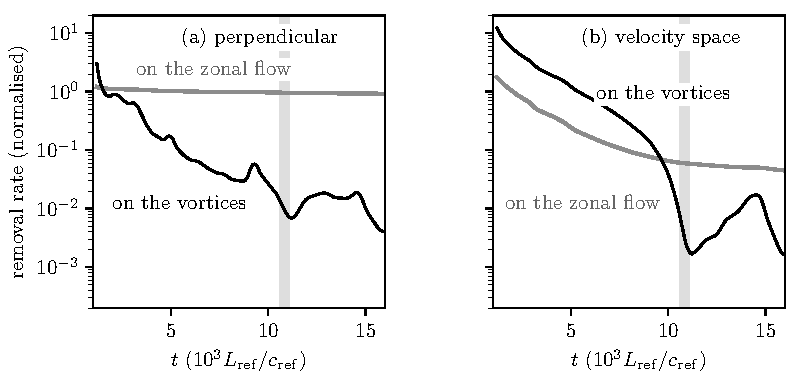
\includegraphics{figures/dissipation.pdf}
\caption{Where the free energy is removed. The rate of removal by (a) the perpendicular and (b) the velocity-space hyperdiffusion, each split into the part that acts on the zonal (\(k_y = 0\); grey) and on the non-zonal (\(k_y\geq1\); black) part of the distribution, in sliding windows of about a hundred breathing periods, in units of the perpendicular removal from the zonal part in the slow phase of the decay; the parallel sink is negligible and is not shown. The grey band marks the collapse. The perpendicular sink belongs to the zonal flow and the velocity-space sink to the vortices.}
\label{fig:dissipation}
\end{figure}

The exchange with the jets behaves as prediction (v) requires. Throughout the slow phase of the decay, the jets supply the vortices with electrostatic energy at a rate that makes up for most of the loss, so the slow decay of \cref{fig:history} is the small difference between two larger rates. As the vortices weaken, and their jets become less unstable, the supply fades, passes through zero, and becomes a drain: once the jets are stable, the vortices give energy back to them, and collapse [see \cref{fig:exchange}(b)]. The restarts follow the same curve: the \(\epsilon = 0.3\) restart has the loss rate of the original run and a smaller supply, and the \(\epsilon = 0.03\) restart has the loss rate of the original run and, once its regrowth is over, a drain. The acceleration of the decay, and its dependence on amplitude, are therefore those of the exchange with the jets, not of the damping. The mean transfer from the jets is also why the zonal flow decays faster while the vortices are large than after they have gone [see \cref{fig:history}(b)].

\subsection{The fluid limit by itself}\label{sec:fluidmodel}

Prediction (vi) is tested by integrating the two-dimensional Euler equation \cref{eq:euler} in the box of the simulation, with the same Fourier modes and the same perpendicular hyperdiffusion,\footnote{The perpendicular hyperdiffusion of the simulation acts on \(h_a\), whose charge moment is proportional to \((1 + \kperp^2\lambdaD^2)\phi\), so in the fluid limit it damps the vorticity at its nominal rate multiplied by \(1 + 1/\kperp^2\lambdaD^2\). With this sink and no other, the fluid model reproduces the measured decay rate of the zonal flow.} starting from the potential of the simulation in the slow phase of the decay (see \cref{fig:euler}). The fluid model reproduces the two counter-propagating vortices, their phase speed, the breathing, and the regrowth of the amplitude tests, which in it proceeds at the full Rayleigh rate. Without the sink, its vortices do not decay. With it, they decay at a rate roughly proportional to the sink, because the sink erodes the corrugation of the jets, and they collapse once small enough. They decay more slowly than in the simulation, however: what the fluid limit lacks is the kinetic loss \(L\).

\begin{figure}
\centering
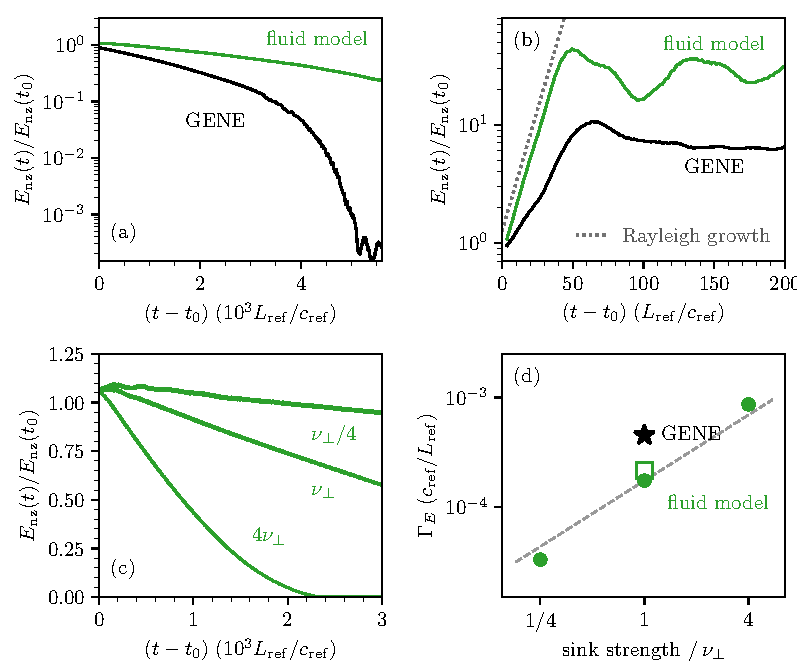
\includegraphics{figures/euler.pdf}
\caption{The two-dimensional fluid model against the kinetic simulation. (a) The non-zonal energy of the simulation (black) and of the fluid model started from its potential at the time \(t_0\) of the amplitude tests (green). (b) The same for the restart with the vortices reduced by \(\epsilon = 0.03\), with growth at the Rayleigh rate (dotted). (c) The fluid model with its perpendicular sink multiplied by four, unchanged, and divided by four. (d) The decay rate of the fluid model against the strength of its sink (circles; the square is at twice and four times the radial resolution), a linear dependence (dashed) and the simulation (star). All curves are running means over ten breathing periods [two in (b)]. A fluid with the perpendicular sink of the simulation reproduces the vortices, their regrowth and a part of their decay; the rest of the damping is kinetic.}
\label{fig:euler}
\end{figure}

\subsection{The collapse}\label{sec:collapse}

The fluid in the cat's eyes turns over many times in the time over which the vortices decay [see \cref{fig:trapping}(a)], which is the condition for the vortices to follow their jets adiabatically (\cref{sec:pendulum}). The decay speeds up as the cat's eyes narrow, and the vortices collapse when the half-width \(w\) of the eyes has fallen to about one grid cell [see \cref{fig:trapping}(b)], which is when the jets become stable [see \cref{fig:rayleigh}(d)]. After the collapse, what is left at \(k_y = 1\) is not a vortex but a weak forced response to the zonal state, supplied by the zonal flow and removed by the perpendicular sink at nearly equal rates.

\begin{figure}
\centering
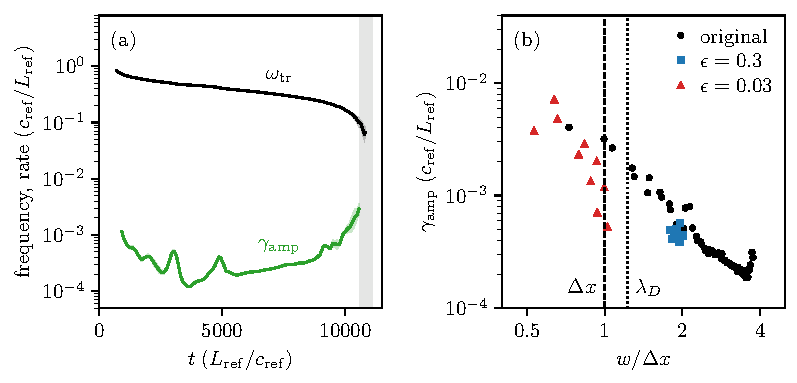
\includegraphics{figures/trapping.pdf}
\caption{Time scales of the vortices and the approach to the collapse. (a) The trapping frequency \(\omtr\) of \cref{eq:trapping} at the critical layer (black) and the amplitude decay rate \(\gammaamp = \GammaE/2\) (green), each as the geometric mean of the two vortices on a band that spans them; \(\gammaamp\) is from sliding fits of the logarithm of the energy of each vortex in windows of about a hundred breathing periods, and the grey band marks the collapse. (b) The decay rate of each vortex, from fits in windows half as long, against the half-width \(w\) of its cat's eye in units of the grid spacing, for the original run (black dots) and for the \(\epsilon = 0.3\) (blue squares) and \(\epsilon = 0.03\) (red triangles) restarts after their regrowth; the dashed and dotted vertical lines mark \(w = \dx\) and \(w = \lambdaD\). The fluid in the cat's eyes turns over many times while the vortices decay, and the decay speeds up as the cat's eyes narrow towards one grid cell, which is also about one Debye length.}
\label{fig:trapping}
\end{figure}

In this simulation, the grid spacing is also about one Debye length, \(\lambdaD\approx1.2\,\dx\), so the corrugation of the jets, the scale at which the vortices cease to be flute-like, and the smallest scale that the grid resolves all coincide. What erodes the corrugation, and so sets the lifetime of the vortices, is therefore not settled by this simulation alone: it may be the perpendicular hyperdiffusion, as in the fluid model of \cref{sec:fluidmodel}, or the vortices themselves, which draw on the corrugation the energy that they lose. The restarts of \cref{sec:runs} are designed to separate the two. If the perpendicular hyperdiffusion erodes the corrugation, the decay should speed up and slow down with it. If the loss is Landau damping, it should not depend on the coefficient of the velocity-space hyperdiffusion. If the collapse is set by the grid, it should move to an energy of the vortices about sixteen times lower when the radial resolution is doubled, while an effect of the Debye scale would not move.

% ===========================================================================
\section{Summary and discussion}\label{sec:summary}
% ===========================================================================

We have given a theory of the breathing vortices of the strongly driven dipole pair-plasma condensate, and of their decay, and tested it against a reduced-box simulation and restarts of it. Let us state what we consider established.

Firstly, at the scale of the box, the jets and the vortices obey the two-dimensional Euler equation \cref{eq:euler}, and the vortices are the unstable mode of Rayleigh's equation \cref{eq:rayleigh} on their jets: it has their frequency, throughout the run, and their radial structure. The jets are unstable because their shear layers are corrugated at the Debye scale.

Secondly, the instability is saturated by trapping: the trapping frequency of the vortices is a constant multiple of the Rayleigh growth rate of their jets, \cref{eq:saturation}, while their energy falls by orders of magnitude, and a vortex that is reduced in amplitude on unchanged jets regrows.

Thirdly, the vortices are damped kinetically and linearly. Their electrostatic energy is converted into entropy at a rate that does not depend on their amplitude, by the streaming of particles along the field line, on which the non-flute part of their potential does work; the entropy is then removed by the velocity-space sink.

Finally, the jets feed the vortices at nearly the rate at which they are damped, as long as they are unstable. The vortices decay because their jets slowly lose their instability, and they collapse when the jets become stable and the exchange with them reverses. A two-dimensional fluid with the same jets has the same vortices, but not their kinetic loss.

The following remain open. We have estimated the kinetic loss, \cref{eq:loss}, but not calculated it from first principles: this requires the non-flute part of the potential from \cref{eq:poisson} and its damping by particles that are resonant with the vortex in the frame of the local flow, both of which are outside the transit-averaged equations. We have no theory of the constant \(\alpha\) of \cref{eq:saturation}, or of the rate at which the corrugation of the jets is eroded, which, with \cref{eq:saturation}, would give the lifetime of the vortices. In the simulation, the corrugation, the Debye length and the grid spacing are all of the same size, and the restarts that separate them are running at the time of writing (\cref{sec:collapse}). In view of this, we do not claim a lifetime for the vortices in physical units, nor that they would decay in a better-resolved or collisional plasma. Whether trapping-saturated shear instability, drained by Landau damping at the Debye scale, is what ultimately limits the lifetime of coherent structures in strongly driven pair-plasma condensates --- and how the answer changes with physical collisions and with the radial scale of the condensate in a device --- appears to be a promising subject for future work.

\section*{Acknowledgements}
The simulations analysed here were carried out on the Cambridge Service for Data Driven Discovery (CSD3).

\section*{Funding}
The authors received no specific funding for this work.

\section*{Declaration of interests}
The authors report no conflict of interest.

\appendix

\IfFileExists{appendices/appE_rayleigh.tex}{% ===========================================================================
\section{From the kinetic equation to Rayleigh's equation}\label{app:rayleigh}
% ===========================================================================

Here we derive, step by step, the fluid equations that govern the vortices, viz., the Euler equation \cref{eq:euler} and Rayleigh's equation \cref{eq:rayleigh}, and then the formula \cref{eq:gamma_rayleigh} for the growth rate of the shear-flow instability of the jets. The starting point is the transit-averaged system \cref{eq:kinetic,eq:poisson}. The only assumption is that the potential is flute-like, i.e., independent of the position \(l\) along the field line, so that \(\phibar = \phi\) in \cref{eq:orbit}; this is the case when \(\kperp\lambdaD\ll1\).

\subsection{The charge moment}\label{app:rayleigh_moment}

The field equation \cref{eq:poisson} involves the distribution functions only through their charge moment, \(\sum_a e_a\intv h_a = e\intv(h_p - h_e)\), so let us find the equation that this moment obeys: we multiply \cref{eq:kinetic} by \(e_a\), integrate over velocities and sum over the two species. Consider the terms of \cref{eq:kinetic} in turn. Firstly, by \cref{eq:poisson}, the charge moment itself is
\begin{equation}
\sum_a e_a\intv h_a = \frac{2n_0e^2}{T}\left(1 - \lambdaD^2\nabla_\perp^2\right)\phi,
\label{eq:Echarge}
\end{equation}
which gives the moment of \(\pt h_a\). Secondly, a flute-like potential does not depend on the velocity, so the bracket commutes with the velocity integral, and the moment of \(\pbrainline{\phi}{h_a}\) is the bracket of \(\phi\) with \cref{eq:Echarge}; since \(\pbrainline{\phi}{\phi} = 0\), only \(-(2n_0e^2\lambdaD^2/T)\pbrainline{\phi}{\nabla_\perp^2\phi}\) survives. Thirdly, the magnetic drifts of the two species are equal and opposite, \(\bar v_{de} = -\bar v_{dp}\), and so are their charges, whence \(e_a\vda = e\bar v_{dp}\) for both, and the moment of the drift term is \(e\,\partial_\alpha\intv\bar v_{dp}(h_p + h_e)\): the drift couples the charge moment to the \textit{sum} of the two distributions. Fourthly, on the right-hand side, \(\sum_a e_a^2\intv f_0/T = 2n_0e^2/T\), so the first term gives \((2n_0e^2/T)\,\pt\phi\). Finally, \((e_af_0/T)\,v_{*a}^T = -\partial_\psi f_0\) is the same for both species, so the gradient drive, multiplied by \(e_a\) and summed, vanishes. Collecting the terms, we get
\begin{equation}
\frac{2n_0e^2}{T}\left[\pt\phi - \lambdaD^2\,\pt\nabla_\perp^2\phi - \lambdaD^2\pbra{\phi}{\nabla_\perp^2\phi}\right] + e\,\partial_\alpha\intv\bar v_{dp}\left(h_p + h_e\right) = \frac{2n_0e^2}{T}\,\pt\phi.
\label{eq:Ecollect}
\end{equation}
The terms \(\pt\phi\) on the two sides cancel: they describe the Boltzmann part of the response, which follows the potential adiabatically and exerts no net effect. What remains, divided by \(-2n_0e^2\lambdaD^2/T\), is \cref{eq:euler}. Three things have dropped out of it, viz., the gradients of the equilibrium, the time derivative of \(\phi\) itself and, apart from the prefactor of the drift term, the Debye length.

The drift term on the right-hand side of \cref{eq:euler} is smaller than the advection terms on its left-hand side by the ratio of the drift speed of a thermal particle to the speed of the vortex relative to the zonal flow, \(|\vda|/|U - c|\), which is very small for the vortices of these notes (\cref{sec:geometry}). Without it, \cref{eq:euler} is the two-dimensional Euler equation of an incompressible, inviscid fluid, written for its streamfunction \(\phi\): the velocity is \((-\partial_\alpha\phi, \partial_\psi\phi)\) in the \((\psi,\alpha)\) plane, \(\nabla_\perp^2\phi\) is the vorticity, and the equation states that the vorticity of each fluid element is conserved as it is carried by the flow.

\subsection{The average along the field line}\label{app:rayleigh_metric}

In a flux tube, the perpendicular Laplacian is \(\nabla_\perp^2 = g^{xx}\partial_\psi^2 + 2g^{xy}\partial_\psi\partial_\alpha + g^{yy}\partial_\alpha^2\), where \(g^{xx} = |\grad\psi|^2\), \(g^{xy} = \grad\psi\bcdot\grad\alpha\) and \(g^{yy} = |\grad\alpha|^2\), in the normalised coordinates of the flux tube, are the metric coefficients; these vary along the field line, whereas a flute-like \(\phi\) and the distributions \(h_a\) do not. Equation \cref{eq:poisson} can therefore hold only on average, and \cref{eq:Echarge} is to be read as its average over the volume of the flux tube, \(\langle\cdot\rangle\equiv\int(\rmd l/B)(\cdot)\big/\!\int\rmd l/B\). (The departure of \(\phi\) from a flute-like function that restores \cref{eq:poisson} at every \(l\) is of relative order \(\kperp^2\lambdaD^2\); it does not affect the motion of the vortices, but it is what damps them, see \cref{sec:loss}.) The derivation of \cref{app:rayleigh_moment} goes through unchanged with \(\nabla_\perp^2\) replaced by its average. In the flux tube of the simulations, \(g^{xy} = 0\), so the vorticity is
\begin{equation}
\zeta = \langle g^{xx}\rangle\,\partial_\psi^2\phi + \langle g^{yy}\rangle\,\partial_\alpha^2\phi,
\qquad
\pt\zeta + \pbra{\phi}{\zeta} = 0.
\label{eq:Evorticity}
\end{equation}
In other words, the fluid is two-dimensional and incompressible, but its vorticity is an anisotropic Laplacian of its streamfunction.

\subsection{Rayleigh's equation and the critical layer}\label{app:rayleigh_equation}

Let the potential be that of a zonal flow, \(\Phi(\psi)\), plus a small wave, \(\phi = \Phi + \operatorname{Re}[\varphi(\psi)\,\rme^{\rmi k\alpha - \rmi\omega t}]\), with \(k > 0\), and let \(U\equiv\partial_\psi\Phi\) be the velocity of the zonal flow, which is in the \(\alpha\) direction. Any \(\Phi(\psi)\) is a steady solution of \cref{eq:Evorticity}, because its vorticity \(\langle g^{xx}\rangle U'\) is also a function of \(\psi\) alone. To first order in the wave, the three terms of \cref{eq:Evorticity} are: the rate of change of the vorticity of the wave, \(-\rmi\omega\,(\langle g^{xx}\rangle\varphi'' - \langle g^{yy}\rangle k^2\varphi)\); its advection by the zonal flow, \(\rmi kU\,(\langle g^{xx}\rangle\varphi'' - \langle g^{yy}\rangle k^2\varphi)\); and the advection of the zonal vorticity by the radial velocity \(-\rmi k\varphi\) of the wave, \(-\rmi k\varphi\,\langle g^{xx}\rangle U''\). Their sum, divided by \(\rmi k\langle g^{xx}\rangle\), is Rayleigh's equation,
\begin{equation}
\left(U - c\right)\left(\varphi'' - k_\text{eff}^2\varphi\right) - U''\varphi = 0,
\qquad
c\equiv\frac{\omega}{k},
\qquad
k_\text{eff}^2\equiv k^2\,\frac{\langle g^{yy}\rangle}{\langle g^{xx}\rangle},
\label{eq:Erayleigh}
\end{equation}
which is \cref{eq:rayleigh} with the metric restored; primes denote derivatives with respect to \(\psi\). It is an eigenvalue problem: for a given jet \(U(\psi)\), periodic solutions \(\varphi\) exist only for special values of the phase speed \(c\), in general complex, and the wave grows at the rate \(\gamma_\text{R}\equiv\operatorname{Im}\omega = k\operatorname{Im}c\).

A \textit{critical layer} is a radius \(\psi_c\) at which the real part of the phase speed equals the speed of the flow, \(U(\psi_c) = \operatorname{Re}c\). The fluid there moves with the wave and so feels a steady, not an oscillating, radial velocity; this is the resonance of the problem. For a neutral wave, \(\operatorname{Im}c = 0\), the coefficient of the highest derivative in \cref{eq:Erayleigh} vanishes at \(\psi_c\), and the equation is singular: by \cref{eq:Erayleigh}, the vorticity of the wave is \(\varphi'' - k_\text{eff}^2\varphi = U''\varphi/(U - c)\), which diverges as \(1/(\psi - \psi_c)\) unless \(U''_c\varphi_c = 0\), the subscript \(c\) denoting evaluation at the critical layer. For a growing wave, there is no singularity, but the vorticity is concentrated in a layer of width \(\gamma_\text{R}/k|U'_c|\) around \(\psi_c\). Once the wave has a finite amplitude, the fluid in this layer is trapped by it and circulates in the cat's eyes of \cref{sec:pendulum}.

\subsection{When is a jet unstable?}\label{app:rayleigh_theorem}

Let us divide \cref{eq:Erayleigh} by \(U - c\), multiply by the complex conjugate \(\varphi^*\) and integrate over one period in \(\psi\), integrating the first term by parts:
\begin{equation}
\int\rmd\psi\left(|\varphi'|^2 + k_\text{eff}^2|\varphi|^2\right) + \int\rmd\psi\,\frac{U''\,(U - c^*)}{|U - c|^2}\,|\varphi|^2 = 0.
\label{eq:Equadratic}
\end{equation}
The imaginary part of \cref{eq:Equadratic} is \(\operatorname{Im}c\int\rmd\psi\,U''|\varphi|^2/|U - c|^2 = 0\). Therefore, a growing wave is possible only if \(U''\) changes sign somewhere, i.e., only if the zonal vorticity \(U'\) has an extremum: this is Rayleigh's inflection-point theorem \citep{Rayleigh1880, DrazinReid2004}. It is a necessary condition, not a sufficient one, as the following example, which is the relevant one here, shows.

Consider a jet that is a single harmonic, \(U = U_0\sin q\psi\). It has inflection points, but \(U'' = -q^2U\), and \cref{eq:Equadratic} becomes \(\int\rmd\psi\,(|\varphi'|^2 + k_\text{eff}^2|\varphi|^2) = q^2\int\rmd\psi\,U(U - c^*)|\varphi|^2/|U - c|^2\). For a growing wave, its imaginary part gives \(\int\rmd\psi\,U|\varphi|^2/|U - c|^2 = 0\), and then its real part, with \(U^2 = |U - c|^2 + 2U\operatorname{Re}c - |c|^2\), gives
\begin{equation}
\int\rmd\psi\left[|\varphi'|^2 + \left(k_\text{eff}^2 - q^2\right)|\varphi|^2\right] = -q^2|c|^2\int\rmd\psi\,\frac{|\varphi|^2}{|U - c|^2}\leq0.
\label{eq:Eharmonic}
\end{equation}
The left-hand side is positive if \(k_\text{eff} > q\). Hence a single-harmonic jet is stable to all waves whose effective wavenumber exceeds that of the jet, which is the case for the box-scale wave in the box of the simulations. This is why the metric factor in \cref{eq:Erayleigh} matters, and why a smooth jet could not, by itself, produce the vortices. The argument fails as soon as \(U''\) is no longer proportional to \(U\). In the simulations, each shear layer between the jets is split into two strips of vorticity [see \cref{fig:rayleigh}(a)], so \(U''\) changes sign within each shear layer, close to the critical layers, and the jets are unstable. How fast the wave then grows is the subject of the next subsection.

\subsection{The growth rate}\label{app:rayleigh_growth}

For a growing wave, \cref{eq:Equadratic} can be written as \(\Dfn(\omega) = 0\), where
\begin{equation}
\Dfn(\omega)\equiv\int\rmd\psi\left(|\varphi'|^2 + k_\text{eff}^2|\varphi|^2\right) - \int\rmd\psi\,\frac{kU''|\varphi|^2}{\omega - kU}.
\label{eq:Edispersion}
\end{equation}
We seek its solution \(\omega = \omega_r + \rmi\gamma_\text{R}\) when the growth is slow, \(\gamma_\text{R}\ll\omega_r\). The second integral is then nearly singular at the critical layers, where \(\omega_r = kU\), and we need the limit of \(1/(x + \rmi\epsilon)\) as \(\epsilon\to0^+\), with \(x = \omega_r - kU\). Since
\begin{equation}
\frac{1}{x + \rmi\epsilon} = \frac{x}{x^2 + \epsilon^2} - \rmi\,\frac{\epsilon}{x^2 + \epsilon^2},
\label{eq:Esplit}
\end{equation}
let us consider the integral of each part against a smooth function \(g(x)\). The first part is odd in \(x\) and equals \(1/x\) for \(|x|\gg\epsilon\), while the contribution of \(|x|\lesssim\epsilon\) vanishes with \(\epsilon\) by symmetry; its integral thus tends to the principal value, \(\PV\!\int\rmd x\,g(x)/x\), i.e., the integral with a symmetric interval around \(x = 0\) excised and then shrunk to zero. The second part is a peak of width \(\epsilon\) and area \(\int\rmd x\,\epsilon/(x^2 + \epsilon^2) = \pi\), so its integral tends to \(\pi g(0)\). Therefore,
\begin{equation}
\frac{1}{x + \rmi0} = \PV\frac{1}{x} - \rmi\pi\,\delta(x),
\label{eq:Eplemelj}
\end{equation}
which is the Landau prescription \citep{Landau1946}. The sign of the infinitesimal imaginary part is not a matter of choice. For a growing wave, \(\operatorname{Im}\omega > 0\) literally. More generally, the response to a disturbance applied at some instant is a superposition of terms \(\rme^{-\rmi\omega t}\) with \(\omega\) on a line that lies above all the singularities in the complex plane, since otherwise the response would precede its cause; real frequencies must, therefore, always be approached from above \citep{Landau1946}.

Using \cref{eq:Eplemelj} in \cref{eq:Edispersion}, and \(\delta(\omega_r - kU) = \sum_c\delta(\psi - \psi_c)/k|U'_c|\), we find that, just above the real axis, \(\Dfn = \Dfn_R + \rmi\Dfn_I\) with
\begin{equation}
\Dfn_R(\omega_r) = \int\rmd\psi\left(|\varphi'|^2 + k_\text{eff}^2|\varphi|^2\right) - \PV\!\int\rmd\psi\,\frac{kU''|\varphi|^2}{\omega_r - kU},
\qquad
\Dfn_I = \pi\sum_c\frac{U''_c\,|\varphi_c|^2}{|U'_c|},
\label{eq:Eparts}
\end{equation}
where the sum is over the critical layers. For small \(\gamma_\text{R}\), we expand \(\Dfn(\omega_r + \rmi\gamma_\text{R})\approx\Dfn_R + \rmi\,(\Dfn_I + \gamma_\text{R}\,\partial_{\omega_r}\Dfn_R)\). Here \(\varphi\) may be held fixed: \cref{eq:Edispersion} is the quadratic form of the operator of \cref{eq:Erayleigh}, which is symmetric, so it is stationary with respect to variations of \(\varphi\) about a solution, and the change of \(\varphi\) with \(\gamma_\text{R}\) enters only at second order. The real part of \(\Dfn = 0\) then determines the frequency, \(\Dfn_R(\omega_r) = 0\), and the imaginary part gives the growth rate, \(\gamma_\text{R} = -\Dfn_I/\partial_{\omega_r}\Dfn_R\), i.e.,
\begin{equation}
\gamma_\text{R} = \pi\,\frac{\sum_c U''_c\,|\varphi_c|^2/|U'_c|}{\partial_{\omega_r}\PV\!\int\rmd\psi\,kU''|\varphi|^2/(\omega_r - kU)},
\label{eq:Egrowth}
\end{equation}
which is \cref{eq:gamma_rayleigh}. The derivative in the denominator must be taken after the principal value. Indeed, differentiating under the integral sign would give \(-\int\rmd\psi\,kU''|\varphi|^2/(\omega_r - kU)^2\), which has a double pole at each critical layer and diverges, whereas, with \(s = kU(\psi)\) as the variable of integration on each side of a layer and \(G(s)\equiv U''|\varphi|^2/|U'|\), the shift \(s\to s + \omega_r\) shows that
\begin{equation}
\partial_{\omega_r}\PV\!\int\rmd s\,\frac{G(s)}{\omega_r - s} = \PV\!\int\rmd s\,\frac{G'(s)}{\omega_r - s},
\label{eq:Ederivative}
\end{equation}
which is finite for any \(G\) that is smooth at \(s = \omega_r\).

Equation \cref{eq:Egrowth} has the structure of Landau's formula for the growth of a plasma wave, with the zonal vorticity gradient \(U''\) at the critical layer in the place of the slope of the distribution function at the phase velocity of the wave. Away from the critical layers, the denominator of \cref{eq:Egrowth} is \(-\int\rmd\psi\,kU''|\varphi|^2/(\omega_r - kU)^2\), i.e., minus a weighted average of the vorticity gradient over the body of the wave. Hence the sign of \(\gamma_\text{R}\): the wave grows if the vorticity gradient at its critical layers is opposite in sign to its average over the body of the wave, and decays otherwise. For a single-harmonic jet, the two have the same sign, in agreement with \cref{eq:Eharmonic}; on jets whose shear layers are split into strips, with the critical layers on the strips, they have opposite signs, and the wave grows. Since the fluid elements at the critical layers are trapped once \(\omtr\) is comparable with \(\gamma_\text{R}\), the growth stops there, which is the origin of the saturation law \cref{eq:saturation}.

We have checked \cref{eq:Egrowth} against the growth rates obtained by solving \cref{eq:Erayleigh} numerically, both for jets of the form \(U\propto\sin q\psi + a\sin3q\psi\), in which the third harmonic splits the shear layers when \(a < -1/27\) and makes the jet unstable to waves with \(k_\text{eff} > q\) once the splitting is pronounced enough, and for the jets of the simulations (\cref{sec:unstable}). In both cases, it gives the correct sign and a growth rate close to the exact one, the difference vanishing with \(\gamma_\text{R}/\omega_r\), as expected of a first-order formula.
}{\section{The fluid limit and Rayleigh's equation}\label{app:rayleigh} (In preparation.)}

\IfFileExists{appendices/appG_trapping.tex}{% ===========================================================================
\section{Trapping, the cat's eye and the saturation of the shear instability}\label{app:trapping}
% ===========================================================================

Here we derive, step by step, the results that determine the amplitude of the vortices: that the motion of a fluid element in the frame of a vortex is Hamiltonian, \cref{eq:hamiltonian}; that near a critical layer it is the motion of a pendulum, \cref{eq:pendulum}, with the trapping frequency and the half-width of \cref{eq:trapping}; and that an instability of the jets stops growing when these trapped orbits form, which gives the saturation law \cref{eq:saturation}. Only classical mechanics and elementary fluid dynamics are needed.

\subsection{Motion in the frame of the vortex}\label{app:trapping_frame}

Across a strong magnetic field, every particle, whatever its charge and its energy, moves at the \exb{} velocity. In the local coordinates \((x, y)\), radial and binormal, this velocity is derived from the streamfunction \(\Psi\), which is the electrostatic potential in suitable units: \(\dot x = -\partial_y\Psi\) and \(\dot y = \partial_x\Psi\). The flow is everywhere tangent to the contours of \(\Psi\), since \(\dot x\,\partial_x\Psi + \dot y\,\partial_y\Psi = 0\), so each fluid element would stay on one contour if \(\Psi\) did not depend on time. For a vortex that travels on a zonal flow, however,
\begin{equation}
\Psi = \Psi_\zon(x) + \Psi_v(x, y - ct),
\label{eq:G_psi}
\end{equation}
where the zonal part gives the flow \(U(x) = \Psi_\zon'(x)\) in the \(y\) direction, and the part due to the vortex depends on time, because the vortex moves at its phase speed \(c\), but only through the combination \(y - ct\), as long as its shape is steady. Let us, then, measure position from a point that travels with the vortex, \(\xi \equiv y - ct\). Since \(\partial_y = \partial_\xi\) and \(\dot\xi = \dot y - c\), we have \(\dot x = -\partial_\xi\Psi_v\) and \(\dot\xi = U(x) + \partial_x\Psi_v - c\), whose right-hand sides are the derivatives of a single function:
\begin{equation}
\dot x = -\partial_\xi\Ham,
\qquad
\dot\xi = \partial_x\Ham,
\qquad
\Ham(x, \xi) \equiv \Psi_\zon(x) + \Psi_v(x, \xi) - cx.
\label{eq:G_ham}
\end{equation}
These are Hamilton's equations, with \(\xi\) in the role of the coordinate and \(x\) in that of its conjugate momentum; the term \(-cx\) is the streamfunction of the uniform flow \(-c\) that an observer moving with the vortex sees. Since \(\Ham\) does not depend on time explicitly, \(\rmd\Ham/\rmd t = \partial_x\Ham\,\dot x + \partial_\xi\Ham\,\dot\xi = 0\): each fluid element stays on one contour of \(\Ham\), viz., on a streamline of the flow as it is seen from the vortex. Equation \cref{eq:G_ham} is \cref{eq:hamiltonian} without its drift term, \(\vda x\), which arises in the same way from the magnetic drift and is negligible for the motion (\cref{sec:geometry}).

\subsection{The pendulum and the cat's eye}\label{app:trapping_pendulum}

Without the vortex, \cref{eq:G_ham} gives \(\dot\xi = U(x) - c\): the fluid that flows faster than the vortex overtakes it, the fluid that flows more slowly falls behind, and the fluid on the line \(x = x_r\), where \(U(x_r) = c\), stays level with it. This line is the critical layer. Let us expand \(\Ham\) about it. With \(X \equiv x - x_r\) and the shear \(S \equiv U'(x_r)\), Taylor's theorem gives \(\Psi_\zon(x) - cx = \text{const} + [U(x_r) - c]X + SX^2/2 + \dots\), in which the term linear in \(X\) vanishes by the definition of \(x_r\). If the vortex varies little in \(x\) over the region of interest, we may also set \(\Psi_v(x, \xi) \approx \Psi_v(x_r, \xi) = -A\cos k\xi\), where \(k\) is the wavenumber of the vortex, \(A > 0\) is its amplitude at the critical layer, and the origin of \(\xi\) has been put at a minimum of \(\Psi_v\). Dropping the constant, we obtain \cref{eq:pendulum} and its equations of motion,
\begin{equation}
\Ham = \frac{S}{2}X^2 - A\cos k\xi,
\qquad
\dot\xi = SX,
\qquad
\dot X = -kA\sin k\xi.
\label{eq:G_pendulum}
\end{equation}
The first equation of motion says that the shear carries an element at the distance \(X\) from the critical layer past the vortex at the relative speed \(SX\); the second, that the vortex pushes the element across the layer. Differentiating the first and substituting the second,
\begin{equation}
\frac{\rmd^2(k\xi)}{\rmd t^2} = -k^2SA\,\sin k\xi,
\label{eq:G_pend_eq}
\end{equation}
which is the equation of a pendulum whose angle is \(k\xi\).

Let us take \(S > 0\) first. The point \(k\xi = 0\), \(X = 0\) is the stable equilibrium of the pendulum, and is called the O-point; for small oscillations about it, \(\sin k\xi\approx k\xi\) in \cref{eq:G_pend_eq}, and the motion is harmonic with the frequency \(\omtr\) given below. The points \(k\xi = \pm\pi\), \(X = 0\) are the unstable equilibrium, the pendulum balanced upside down, and are called X-points. The other orbits follow from the conservation of \(\Ham\), whose value is \(-A\) at the O-point and \(+A\) at the X-points. An orbit with \(\Ham < A\) cannot reach \(k\xi = \pm\pi\), where \cref{eq:G_pendulum} would require \(SX^2/2 = \Ham - A < 0\); it goes round the O-point on a closed curve and is said to be trapped. An orbit with \(\Ham > A\) has \(SX^2/2 = \Ham + A\cos k\xi \geq \Ham - A > 0\), so \(X\) never changes sign: the element stays on one side of the critical layer and overtakes the vortex, or is overtaken by it, for ever. The boundary between the two families is the separatrix, \(\Ham = A\), on which \(SX^2/2 = A(1 + \cos k\xi) = 2A\cos^2(k\xi/2)\). Its two arcs, \(X = \pm w\cos(k\xi/2)\), meet at the X-points and enclose a lens-shaped region of trapped fluid, the cat's eye [see \cref{fig:cartoon}(a) and \cref{fig:geometry}(b)], where
\begin{equation}
\omtr = |k|\sqrt{|S|A},
\qquad
w = 2\sqrt{\frac{A}{|S|}}
\label{eq:G_trapping}
\end{equation}
are the trapping frequency and the half-width of the eye at its widest, i.e., \cref{eq:trapping}. Both scale as \(A^{1/2}\). The approximations made in \cref{eq:G_pendulum} hold if \(\Psi_v\) and the shear change little over the distance \(w\).

Two further properties of these orbits will be needed. Firstly, the trapped orbits do not all have the same period: it is \(2\pi/\omtr\) at the centre of the eye and increases outwards, becoming infinite on the separatrix, because a pendulum released from its inverted position takes for ever to leave it. Any pattern carried by the fluid inside the eye is therefore wound into an ever finer spiral. Secondly, if \(S < 0\), the right-hand side of \cref{eq:G_pend_eq} changes sign, so the O-point is at \(k\xi = \pi\) and the X-points are at \(k\xi = 0\), while \cref{eq:G_trapping} holds as written. A jet has \(S > 0\) on one of its flanks and \(S < 0\) on the other, so a vortex whose phase is the same across the jet has its two rows of eyes displaced from each other by half a wavelength, as in \cref{fig:cartoon}(a).

When the variation of the vortex in \(x\) cannot be neglected, the same reasoning applies to the full \(\Ham\). An equilibrium is a point where \(\partial_x\Ham = \partial_\xi\Ham = 0\). Expanding \cref{eq:G_ham} to first order in the displacements \((\delta x, \delta\xi)\) from it gives \(\delta\dot x = -\Ham_{x\xi}\,\delta x - \Ham_{\xi\xi}\,\delta\xi\) and \(\delta\dot\xi = \Ham_{xx}\,\delta x + \Ham_{x\xi}\,\delta\xi\), where the subscripts denote second derivatives at the equilibrium, and solutions proportional to \(\rme^{\lambda t}\) exist if \(\lambda^2 = \Ham_{x\xi}^2 - \Ham_{xx}\Ham_{\xi\xi}\). If this is negative, the neighbouring orbits circle the equilibrium, which is an O-point, at the frequency \(\omtr\) given by \(\omtr^2 = \Ham_{xx}\Ham_{\xi\xi} - \Ham_{x\xi}^2\); if it is positive, they leave it exponentially, and it is an X-point. For \cref{eq:G_pendulum} at its O-point, \(\Ham_{xx} = S\), \(\Ham_{\xi\xi} = k^2A\) and \(\Ham_{x\xi} = 0\), and \cref{eq:G_trapping} is recovered.

\subsection{Saturation of the instability}\label{app:trapping_saturation}

Suppose now that the jets are unstable, i.e., that Rayleigh's equation \cref{eq:rayleigh} has a mode that grows at the rate \(\gamma_\text{R}\) (\cref{sec:euler}). The linear calculation that gives \(\gamma_\text{R}\) follows each fluid element along the path that it would take without the wave, viz., \(X = \text{const}\) and \(\xi = \xi_0 + SXt\) by \cref{eq:G_pendulum}, and computes the small radial displacement \(\delta X\) that the wave adds to it. For a wave of amplitude \(A(t)\propto\rme^{\gamma_\text{R}t}\), integrating the last of \cref{eq:G_pendulum} along this path from the distant past gives
\begin{equation}
\delta X = -k\int_{-\infty}^{t}A(t')\sin\!\left(k\xi_0 + kSXt'\right)\rmd t'
= -kA(t)\operatorname{Im}\frac{\rme^{\rmi k\xi}}{\gamma_\text{R} + \rmi kSX},
\label{eq:G_displacement}
\end{equation}
whose magnitude is at most \(kA/(\gamma_\text{R}^2 + k^2S^2X^2)^{1/2}\). The meaning of \cref{eq:G_displacement} is as follows. An element at the distance \(X\) from the critical layer sees the wave at the frequency \(kSX\), Doppler shifted by its motion past the vortex. If \(|kSX|\gg\gamma_\text{R}\), the push that it receives reverses many times while the wave grows by a factor of \(\rme\), and its effect averages out. If \(|kSX|\lesssim\gamma_\text{R}\), the push has the same sign for a whole growth time. It is these elements, displaced steadily across the gradient of the zonal vorticity, that pass energy from the jet to the wave [cf.\ \cref{eq:gamma_rayleigh}]. They occupy a resonant layer about the critical layer, of half-width \(X_\gamma \equiv \gamma_\text{R}/|k||S|\).

The true paths, however, are those of \cref{eq:G_pendulum}, and the unperturbed path is a good approximation to them only as long as the wave cannot turn an element round within one growth time, i.e., as long as \(\omtr\ll\gamma_\text{R}\). By \cref{eq:G_trapping}, the same condition can be written as
\begin{equation}
\frac{w}{X_\gamma} = \frac{2\omtr}{\gamma_\text{R}} \ll 1,
\label{eq:G_ratio}
\end{equation}
viz., the cat's eye must be a thin sliver inside the resonant layer. As the wave grows, \(\omtr\propto A^{1/2}\) grows with it, until \(\omtr\) is comparable with \(\gamma_\text{R}\). The eye has then swallowed the resonant layer, and the elements that were feeding the wave go round the eye in about the time that the wave needs to grow. An element that goes round gives the wave nothing on average: on one half of its orbit it moves across the layer one way, and on the other half it comes back. Moreover, since the orbits have different periods, the vorticity inside the eye is wound up and, after a few turns, is uniform on average along each closed streamline, so the gradient that drove the instability has been flattened where it mattered. The growth stops. This is the argument of \citet{ONeil1965} for a plasma wave and the particles that resonate with it; for a shear flow, it is the theory of the nonlinear critical layer \citep{Stewartson1978, WarnWarn1978}.

The wave therefore saturates at the amplitude for which
\begin{equation}
\omtr = \alpha\,\gamma_\text{R},
\qquad\text{i.e.,}\qquad
A = \frac{\alpha^2\gamma_\text{R}^2}{k^2|S|},
\label{eq:G_saturation}
\end{equation}
where \(\alpha\) is a pure number and \cref{eq:G_trapping} has been used. This is \cref{eq:saturation}. The argument fixes how the amplitude scales with the growth rate, the wavenumber and the shear, which is what can be tested, but not the value of \(\alpha\): `comparable' covers anything from a fraction of a trapping period, \(2\pi/\omtr\), to several periods, and the answer depends on how the vorticity is distributed near the layer. We do not derive \(\alpha\); it is measured in \cref{fig:saturation}.

Finally, let us explain why the amplitude continues to obey \cref{eq:G_saturation} while the jets change. Here \(\gamma_\text{R}\) is the growth rate on the jets as they are at a given time, so \cref{eq:G_saturation} relates two quantities that can be measured independently. The trapping time \(1/\omtr\) and the growth time \(1/\gamma_\text{R}\) are comparable by \cref{eq:G_saturation}, and both are much shorter than the time over which the jets, and hence \(\gamma_\text{R}\), change. If the amplitude is below the level \cref{eq:G_saturation} of the current jets, the eye is narrower than the resonant layer, and the wave grows again, at a rate of order \(\gamma_\text{R}\), until the elements that feed it are trapped once more; this takes a few growth times, an instant on the time scale of the jets, and it is what happens when the vortices are reduced artificially [see \cref{fig:euler}(b)]. If, on the other hand, \(\gamma_\text{R}\) falls, the level that trapping can sustain falls with it, and the weak damping of the vortices (\cref{sec:dissipation}), which acts all the time, brings the amplitude down to that level, provided that the jets change more slowly than the vortices are damped. In other words, the amplitude follows \(\gamma_\text{R}(t)\) adiabatically, as in \cref{fig:saturation}(a), until \(\gamma_\text{R}\) vanishes, the jets are stable, and nothing sustains the vortices.
}{\section{Trapping and the saturation of the instability}\label{app:trapping} (In preparation.)}

\IfFileExists{appendices/appH_landau.tex}{% ===========================================================================
\section{Landau damping of the non-flute part of a vortex}\label{app:landau}
% ===========================================================================

Here we derive the rate \(\mathcal{L}\) at which a vortex loses electrostatic energy to entropy, \cref{eq:loss} of \cref{sec:loss}. The calculation has four steps: the motion of a particle along the field line, the response of the particles to a potential that varies along the line, the part of the vortex potential that does so, and the work that this part does on the particles.

\subsection{Motion along the field line}

To lowest order, a particle slides along its field line with its energy \(\varepsilon = mv^2/2\) and its pitch-angle variable \(\lambda = v_\perp^2/Bv^2\) conserved, so its parallel velocity is
\begin{equation}
\frac{\rmd l}{\rmd t} = v_\parallel = \pm v\sqrt{1 - \lambda B(l)}.
\label{eq:Horbit}
\end{equation}
If \(\lambda B < 1\) everywhere, the particle is \textit{passing}: it travels the whole length of the field line and, in the periodic flux tube, comes round again. Otherwise it is \textit{trapped}: it is reflected where \(\lambda B(l) = 1\) and bounces between two such points. Either way the motion is periodic. Its period is \(\tau = \hat\tau(\lambda)/v\) for a passing particle and \(\tau = 2\hat\tau(\lambda)/v\) for a trapped one, with \(\hat\tau\) the integral defined in \cref{eq:orbit}, and we call \(\omega_\tau \equiv 2\pi/\tau\) the \textit{orbit frequency}. It is proportional to \(v\), so there are particles with every orbit frequency from zero upwards; for a thermal particle, \(\omega_\tau\) is of the order of the transit frequency, viz., the thermal speed divided by the length of the field line. We describe the position of a particle on its orbit by the angle \(\theta = \omega_\tau t\), which increases by \(2\pi\) per period, so that any function of position along the line is, for that particle, a periodic function of \(\theta\). In particular, the potential that the particle sees is
\begin{equation}
\varphi\left(l(\theta)\right) = \sum_{n=-\infty}^{\infty}\varphi_n\,\rme^{\rmi n\theta},
\qquad
\varphi_n(\lambda) = \frac{1}{2\pi}\oint\varphi\left(l(\theta)\right)\rme^{-\rmi n\theta}\,\rmd\theta .
\label{eq:Hharmonics}
\end{equation}
The harmonic \(n = 0\) is the orbit average \(\overline\varphi\) of \cref{eq:orbit}. If the potential is flute-like, i.e., the same at every point of the field line, all the other harmonics vanish. The harmonics \(\varphi_n\) depend on \(\lambda\), which fixes the shape of the orbit, but not on the speed.

\subsection{Response of the particles}

Let the vortex be \(\phi = \varphi(x, l)\,\rme^{\rmi ky - \rmi\omega t}\). Its particles are carried in \(y\) by the zonal flow \(U(x)\), so that, at the radius \(x\), they see the vortex oscillate at the Doppler-shifted frequency
\begin{equation}
\wt(x) = \omega - kU(x),
\label{eq:Hdoppler}
\end{equation}
which vanishes at the critical layers and is largest in the middle of the jet. Following a particle along its orbit, the non-adiabatic part of its distribution, \(g_a\rme^{\rmi ky - \rmi\omega t}\), obeys
\begin{equation}
\left(\frac{\rmd}{\rmd t} - \rmi\wt\right)g_a = -\rmi\wt\,\frac{e_af_0}{T}\,\varphi\left(l(t)\right),
\label{eq:Hkinetic}
\end{equation}
where \(\rmd/\rmd t\) is the rate of change along the orbit \cref{eq:Horbit}. This is \cref{eq:kinetic} before the average over the orbit has been taken: the left-hand side is the change of \(g_a\) seen by the moving particle in the frame of the zonal flow, and the right-hand side is the rate at which the potential changes the energy of a particle, \(e_a\,\partial\phi/\partial t\), times the slope \(-f_0/T\) of the Maxwellian in energy. We have left out the magnetic drift, which is smaller than \(\wt\) by orders of magnitude, and the gradients of the equilibrium, whose contributions to the charge are equal and opposite for the two species.

Since everything in \cref{eq:Hkinetic} is periodic in \(\theta\), and \(\rmd/\rmd t = \omega_\tau\,\partial/\partial\theta\), each harmonic can be solved for separately:
\begin{equation}
g_a = \frac{e_af_0}{T}\sum_n\frac{\wt}{\wt - n\omega_\tau}\,\varphi_n\,\rme^{\rmi n\theta}.
\label{eq:Hresponse}
\end{equation}
The term \(n = 0\) is the response to the orbit-averaged potential and is all that the transit-averaged equations of \cref{sec:equations} retain. The other terms are resonant: the particles for which \(n\omega_\tau = \wt\), i.e., those that complete \(n\) orbits in one period of the vortex as they see it, respond without limit. As in any such problem, the resonance is resolved by causality. A response that has been built up from the past is obtained by giving \(\omega\) a small positive imaginary part, and then
\begin{equation}
\frac{1}{\wt - n\omega_\tau + \rmi0} = \PV\frac{1}{\wt - n\omega_\tau} - \rmi\pi\,\delta\left(\wt - n\omega_\tau\right),
\label{eq:Hplemelj}
\end{equation}
where \(\PV\) denotes the principal value. To see this, replace \(\rmi0\) by \(\rmi\epsilon\): the imaginary part of \(1/(X + \rmi\epsilon)\) is \(-\epsilon/(X^2 + \epsilon^2)\), a peak of width \(\epsilon\) and area \(\pi\), which becomes \(-\pi\delta(X)\) as \(\epsilon\to0\), while the real part, \(X/(X^2 + \epsilon^2)\), is \(1/X\) with the neighbourhood of \(X = 0\) cut out symmetrically. The first term of \cref{eq:Hplemelj} is a response in phase with the potential, which exchanges no energy on average. The second is a quarter of a period out of phase: it is the resonant particles, and only they, that take energy from the potential. This is Landau damping \citep{Landau1946}, with the orbit frequency in place of the frequency \(k_\parallel v_\parallel\) of a particle streaming along a straight field.

The charge density that the two species carry between them follows by integrating \cref{eq:Hresponse} over velocities. In the units of \cref{eq:poisson}, the right-hand side of that equation becomes
\begin{equation}
\frac{1}{2n_0}\intv\left(h_p - h_e\right) = \frac{e}{T}\,\rho[\varphi],
\qquad
\rho[\varphi](l) \equiv \frac{1}{n_0}\intv f_0\sum_n\frac{\wt}{\wt - n\omega_\tau + \rmi0}\,\varphi_n\,\rme^{\rmi n\theta(l)},
\label{eq:Hrho}
\end{equation}
where \(\theta(l)\) is the orbit angle at which the particle of velocity \(\vv\) passes the point \(l\). For a flute-like potential, only \(n = 0\) survives and \(\rho[\varphi] = \varphi\): the particles screen a flute-like potential exactly as a Boltzmann response would, and exchange no energy with it.

\subsection{The non-flute part of the vortex}

A vortex cannot be exactly flute-like, because the left-hand side of \cref{eq:poisson} is not. In the flux tube, \(\nabla_\perp^2 = g^{xx}(l)\,\partial_x^2 + g^{yy}(l)\,\partial_y^2\), where the metric coefficients \(g^{xx}\) and \(g^{yy}\) measure how the distances between neighbouring field lines change along them, and they do not vary in proportion to each other. Let us write \(\varphi = \varphi_0(x) + \varphi_1(x, l)\), where \(\varphi_0\) is the average of \(\varphi\) along the field line, weighted by the volume of the flux tube, and \(\varphi_1\) is the small non-flute part. The charge moment of the kinetic equation, taken at one point of the field line, states that the charge \(-\lambdaD^2\nabla_\perp^2\phi\) of a fluid element changes only through the divergence of the current along the line. Averaged along the line, this divergence vanishes, and what remains is the Euler equation of \cref{app:rayleigh}: the average charge, \(-\lambdaD^2(\langle g^{xx}\rangle\partial_x^2 + \langle g^{yy}\rangle\partial_y^2)\phi\), is carried with the flow. The part of the charge that varies along the line,
\begin{equation}
-\lambdaD^2\left[\left(g^{xx} - \langle g^{xx}\rangle\right)\partial_x^2 + \left(g^{yy} - \langle g^{yy}\rangle\right)\partial_y^2\right]\phi,
\label{eq:Hcharge}
\end{equation}
is carried with the same flow, and since the average charge is conserved, the rate of change of \(\partial_x^2\phi\) following the flow is \(-\langle g^{yy}\rangle/\langle g^{xx}\rangle\) times that of \(\partial_y^2\phi\), which, for the vortex, is \(\rmi\wt k^2\varphi_0\). Hence the charge \cref{eq:Hcharge} changes at the rate \(\rmi\wt\,S(l)\,\varphi_0\), with
\begin{equation}
S(l) = k^2\lambdaD^2\,s(l),
\qquad
s(l) \equiv \langle g^{yy}\rangle\left[\frac{g^{xx}(l)}{\langle g^{xx}\rangle} - \frac{g^{yy}(l)}{\langle g^{yy}\rangle}\right].
\label{eq:Hsource}
\end{equation}
A charge that varies along the line can change only through currents along the line, and only a potential that varies along the line drives such currents. The charge that \(\varphi_1\) induces is, in the units of \cref{eq:poisson}, the response \cref{eq:Hrho} less the Boltzmann part, viz., \(\rho[\varphi_1] - \varphi_1\), and it changes at the rate \(-\rmi\wt\,(\rho[\varphi_1] - \varphi_1)\). Equating the two rates, we find
\begin{equation}
\varphi_1 - \rho[\varphi_1] = S(l)\,\varphi_0 ,
\label{eq:Hfield}
\end{equation}
which is the part of \cref{eq:poisson} that varies along the line. In other words, the non-flute part of a vortex is forced by its flute-like part through the geometry of the field, in proportion to \(k^2\lambdaD^2\); it does not depend on the radial structure of the vortex, and it is linear in its amplitude. Writing \(\varphi_1 = k^2\lambdaD^2\,\chi(l;\wt)\,\varphi_0\), we have
\begin{equation}
\chi - \rho[\chi] = s(l),
\label{eq:Hchi}
\end{equation}
a linear equation along the field line whose only parameter is the ratio of \(\wt\) to the transit frequency. We solve it numerically, by expanding \(\chi\) in Fourier harmonics along the line and computing the orbits \cref{eq:Horbit} and the harmonics \cref{eq:Hharmonics} in the magnetic field of the flux tube. Because of the resonant term of \cref{eq:Hplemelj}, \(\chi\) is complex: the non-flute part of the vortex lags behind the forcing.

\subsection{The loss of energy}

The electrostatic energy changes at the rate \(\int\phi\,\partial_t\varrho\), where \(\varrho\) is the charge density. The part of \(\partial_t\varrho\) that is due to the motion of the particles along the field line is minus the divergence of the parallel current, so the corresponding change of energy is minus the work done by the parallel electric field on the particles. Only \(\varphi_1\) has a parallel electric field, and, by \cref{eq:Hplemelj}, only the resonant particles absorb work on average. Carrying out the average over the orbits with \cref{eq:Hresponse}, we find that, per unit volume, the two species together absorb the power
\begin{equation}
\frac{\pi n_0e^2}{T}\left\langle\!\!\left\langle\,\wt^2\sum_{n\neq0}|\varphi_{1,n}|^2\,\delta\left(\wt - n\omega_\tau\right)\right\rangle\!\!\right\rangle
= \frac{n_0e^2}{T}\,\wt\,\operatorname{Im}\left\langle\varphi_1^*\,S\,\varphi_0\right\rangle,
\label{eq:Hpower}
\end{equation}
where the double angle brackets denote the average over the Maxwellian and over the flux tube, the single ones the volume-weighted average along the field line, and the equality follows by multiplying \cref{eq:Hfield} by \(\varphi_1^*\), averaging, and taking the imaginary part. The left-hand side is manifestly positive: every resonance damps. The right-hand side expresses the same power through the lag of \(\varphi_1\) behind its forcing. With \cref{eq:Hchi}, it is \(k^4\lambdaD^4\,|\varphi_0|^2\,(n_0e^2/T)\,\Dfn(\wt)\), where
\begin{equation}
\Dfn(\wt) \equiv -\wt\left\langle s(l)\operatorname{Im}\chi(l;\wt)\right\rangle \geq 0
\label{eq:Hdissipation}
\end{equation}
is a function of the Doppler-shifted frequency that the magnetic geometry fixes once and for all [see \cref{fig:landau}(a)]. It vanishes as \(\wt\to0\), where the particles average over the field line many times in a period of the vortex and the transit-averaged description applies; it is largest where \(\wt\) is a few times the transit frequency; and it falls again at large \(\wt\), where few particles are fast enough to resonate.

Finally, we integrate over the radius and divide by the electrostatic energy of the vortex, \((n_0e^2\lambdaD^2/2T)\int\rmd x\,(\langle g^{xx}\rangle|\partial_x\varphi_0|^2 + \langle g^{yy}\rangle k^2|\varphi_0|^2)\) per unit volume of the flux tube and unit length in \(y\). The result is
\begin{equation}
\frac{\mathcal{L}}{\Enz} = 2\,k^2\lambdaD^2\,
\frac{\displaystyle k^2\int\rmd x\,|\varphi_0|^2\,\Dfn\!\left(\omega - kU\right)}
{\displaystyle\int\rmd x\left(\langle g^{xx}\rangle|\partial_x\varphi_0|^2 + \langle g^{yy}\rangle k^2|\varphi_0|^2\right)},
\label{eq:Hrate}
\end{equation}
summed over the two vortices in the numerator and in the denominator. It contains no adjustable parameter: given the flute-like structure of the vortices and the jets, which are those of the Rayleigh problem of \cref{app:rayleigh}, it is fixed by the geometry of the field.

Three properties of \cref{eq:Hrate} can be tested. Firstly, it is independent of the amplitude of the vortex. Secondly, it is of the order of \(k^2\lambdaD^2\) times the transit frequency, so it is small, and the smaller the longer the vortex is compared with the Debye length. Thirdly, the dissipative response, \(\Dfn\), is a universal function of the local Doppler-shifted frequency, on which measurements at different radii, on either vortex and at different times must all fall.
}{\section{Landau damping of the non-flute part of a vortex}\label{app:landau} (In preparation.)}

\bibliographystyle{jpp}
\bibliography{notes}

\end{document}
